%%%%%%%%%%%%%%%%%%%%%%%%%%%%%%%%%%%%%%%%%%%%%%%%%%%%%%%%%%%%%%%%%%%%%%%%%%%%%%%%%%%%%%%%%%%%%%%%%%%%%%%%%%%%%%%%%%%%%%%%%%%%%%%%%%%%%%%%%%%%%%%%%%%%%%%%%%%
% This is just an example/guide for you to refer to when submitting manuscripts to Frontiers, it is not mandatory to use Frontiers .cls files nor frontiers.tex  %
% This will only generate the Manuscript, the final article will be typeset by Frontiers after acceptance.   
%                                              %
%                                                                                                                                                         %
% When submitting your files, remember to upload this *tex file, the pdf generated with it, the *bib file (if bibliography is not within the *tex) and all the figures.
%%%%%%%%%%%%%%%%%%%%%%%%%%%%%%%%%%%%%%%%%%%%%%%%%%%%%%%%%%%%%%%%%%%%%%%%%%%%%%%%%%%%%%%%%%%%%%%%%%%%%%%%%%%%%%%%%%%%%%%%%%%%%%%%%%%%%%%%%%%%%%%%%%%%%%%%%%%

%%% Version 3.4 Generated 2018/06/15 %%%
%%% You will need to have the following packages installed: datetime, fmtcount, etoolbox, fcprefix, which are normally inlcuded in WinEdt. %%%
%%% In http://www.ctan.org/ you can find the packages and how to install them, if necessary. %%%
%%%  NB logo1.jpg is required in the path in order to correctly compile front page header %%%

\documentclass[utf8]{frontiersSCNS} % for Science, Engineering and Humanities and Social Sciences articles
%\documentclass[utf8]{frontiersHLTH} % for Health articles
%\documentclass[utf8]{frontiersFPHY} % for Physics and Applied Mathematics and Statistics articles

%\setcitestyle{square} % for Physics and Applied Mathematics and Statistics articles
\usepackage{url,hyperref,lineno,microtype,subcaption}
\usepackage[onehalfspacing]{setspace}

\definecolor{light-gray}{gray}{0.95}	
\definecolor{LightCyan}{rgb}{0.88,1,1}
\definecolor{Yellow}{rgb}{1,1,0.3}
\definecolor{light-green}{rgb}{0.5,1,0.5}
\definecolor{light-blue}{rgb}{0.4,0.8,1}
\definecolor{light-yellow}{rgb}{1,0.95,0.8}
\definecolor{dark-blue}{rgb}{0.3,0.8,1}
\usepackage{tablefootnote}
\renewcommand{\thefootnote}{\fnsymbol{footnote}}
\usepackage{framed} % Framing content
\usepackage{multicol} % Multiple columns environment
\usepackage{pdflscape}
\usepackage{tabularx}
\usepackage{color, colortbl}

%\linenumbers


% Leave a blank line between paragraphs instead of using \\



\def\keyFont{\fontsize{8}{11}\helveticabold }
\def\firstAuthorLast{Nice {et~al.}} %use et al only if is more than 1 author
\def\Authors{Kerry~A.~Nice\,$^{1,*}$, Matthias Demuzere\,$^{2}$, Andrew Coutts\,$^{3}$ and Nigel Tapper\,$^{3}$}
% Affiliations should be keyed to the author's name with superscript numbers and be listed as follows: Laboratory, Institute, Department, Organization, City, State abbreviation (USA, Canada, Australia), and Country (without detailed address information such as city zip codes or street names).
% If one of the authors has a change of address, list the new address below the correspondence details using a superscript symbol and use the same symbol to indicate the author in the author list.
\def\Address{$^{1}$Transport, Health, and Urban Design Hub, Faculty of Architecture, Building, and Planning, University of Melbourne, Australia.
$^{2}$Ruhr University Bochum, Germany. 
$^{3}$School of Earth, Atmosphere and Environment, Monash University, Clayton, VIC 3800, Australia. }
% The Corresponding Author should be marked with an asterisk
% Provide the exact contact address (this time including street name and city zip code) and email of the corresponding author
\def\corrAuthor{Kerry A. Nice}

\def\corrEmail{kerry.nice@unimelb.edu.au}




\begin{document}
\onecolumn
\firstpage{1}

\title[Present day and future urban cooling enabled by integrated water management in Australia]{Present day and future urban cooling enabled by integrated water management in Australia} 

\author[\firstAuthorLast ]{\Authors} %This field will be automatically populated
\address{} %This field will be automatically populated
\correspondance{} %This field will be automatically populated

\extraAuth{}% If there are more than 1 corresponding author, comment this line and uncomment the next one.
%\extraAuth{corresponding Author2 \\ Laboratory X2, Institute X2, Department X2, Organization X2, Street X2, City X2 , State XX2 (only USA, Canada and Australia), Zip Code2, X2 Country X2, email2@uni2.edu}


\maketitle


\begin{abstract}

%%% Leave the Abstract empty if your article does not require one, please see the Summary Table for full details.
\section{}
Statistical analysis of the future climate data using historical data shows that future warming is nuanced, with changes variable in both time and place, and with extremes becoming more pronounced in future. We have developed a unique approach to morph the future climate data onto historical data (derived from the ERA5 Reanalysis product) for the 2010-2020 period.  Additionally, we use locally appropriate Local Climate Zones (LCZs) for Australian cities, resulting from a holistic and global approach that is universally adopted by the urban climate modelling community. 

We undertook a review of a number of Government policy documents on the implementation of integrated water management (IWM) (tree cover and area of deep soil targets). Using this, along with professional judgement, we developed scenarios for implementation of moderate and high levels of IWM across each of the Australian LCZs that are consistent with these existing published guidelines. We have also developed a methodology that allows urban climate data gathered at the LCZ level to be aggregated to the statistical area (SA4) and city-wide levels.

We have tested and made improvements to TARGET (The Air temperature Response to Green infrastructure Evaluation Tool) and used the model to provide detailed climate information on the climate benefits of various IWM interventions for both the historical ERA5 (2010-2020) data and for future climate in 2030 and 2050 under different shared socioeconomic pathways (SSPs).  This has been done for nine Australian cities across a range of climatic environments and the data have now been provided to the health modelling team.


\tiny
 \keyFont{ \section{Keywords:} keyword, keyword, keyword, keyword, keyword, keyword, keyword, keyword} %All article types: you may provide up to 8 keywords; at least 5 are mandatory.
\end{abstract}

\section{Introduction}

Cities are hot. Climate change will make them hotter. Hot cities are dangerous. How do we cool them down?

IWM is defined by \cite{GWP2000} as `a process which promotes the coordinated development and management of water, land and related resources, in order to maximise the resultant economic and social welfare in an equitable manner without compromising the sustainability of vital ecosystems'.

Integrated Water Management (IWM) is a thing. Water enables more vegetation. Vegetation can promote cooling. Many local governments have plans to add more vegetation and can utilise IWM.

WSUD uses IWM,
WSUD has many benefits, 
water savings
flood protection
waterway/pollution protections
increased green space/canopy
 \citep{Whiteoak2019b}
 \citep{Renouf2020a}

Because we have IWM, we can test different scenarios to transform cities both in the present and in the future. These involve increasing vegetation and reductions of hard impervious surfaces. 

Here is a bunch of stuff about how that can make cities cooler.

To quantify and compare scenarios, we need to model them. TARGET \citep{Broadbent2019} is a model. Here's what it does. Here is what it will tell us about the scenarios.

So, we can model present day conditions and projected future ones. 

The question then is can we quantify the benefits of IWM in terms of urban cooling in a range of Australian cities under present day and future climate change scenarios.






\section{Methods}\label{sec:methods}


To run TARGET, two sources of information are required: 1) meteorological time series of air temperature, humidity, wind speed, air pressure, and incoming short- and longwave radiation, and 2) gridded land cover fractions that include percentages of roof, road, water, concrete, vegetation (i.e., trees), dry grass, and irrigated grass. 

Since TARGET needs to be applied over seven capital cities (Adelaide, Brisbane, Canberra, Darwin, Melbourne, Perth, and Sydney) and two regional centres (Albury-Wodonga and Townsville), which do not all have the required input data readily available, these datasets are sourced from generic and state-of-the-art data sources and re-structured to fit the requirements of this project. 

\subsection{Meteorological forcing and climate change data}\label{sec:forcing}




%data is superimposed onto present day time series via a "morphing" process. This technique refers to the application of a shift (in mean) and a stretch (in minimum and maximum) of the observed time series, to change both the mean and the variance \citep{Belcher2005,Pulkkinen2021}. For each month, a minimum, median, and maximum air temperature change, and rainfall are computed as the ensemble median over all CMIP6 models and future periods (i.e. 2030 and 2050).



Historical meteorological data are extracted from the ERA5 reanalysis product \citep{Hersbach2020}, provided by ECMWF (European Centre for Medium-Range Weather Forecasts), for the period 2010-2020 and for all nine capital cities and regional centres (see Figure \ref{fig:mel_era5} for Melbourne example). All required TARGET input variables are available at an hourly temporal resolution and represent the average background meteorology for a grid cell of $\sim$30 $\times$ 30 km. ERA5 combines vast amounts of historical observations into global estimates using advanced modelling and data assimilation systems and is to date the best available reanalysis product. We have used ERA5 data rather than Bureau of Meteorology (BoM) data for several reasons. The ERA5 data are a synthesis of observational (BoM) and modelling data that best represent the climate across the urban location of interest, rather than one observational location usually representing a rural environment outside of the urban centre. The data are available hourly and most critically include data (e.g., radiation) required to run TARGET that are not available from the BoM observations. When processed through TARGET, the ERA5 data will give a much better representation of the urban climate than is possible with the original BoM observations. The procedure we have pioneered can now be transferred to any other location in Australia and around the world.

\begin{figure}
\centering
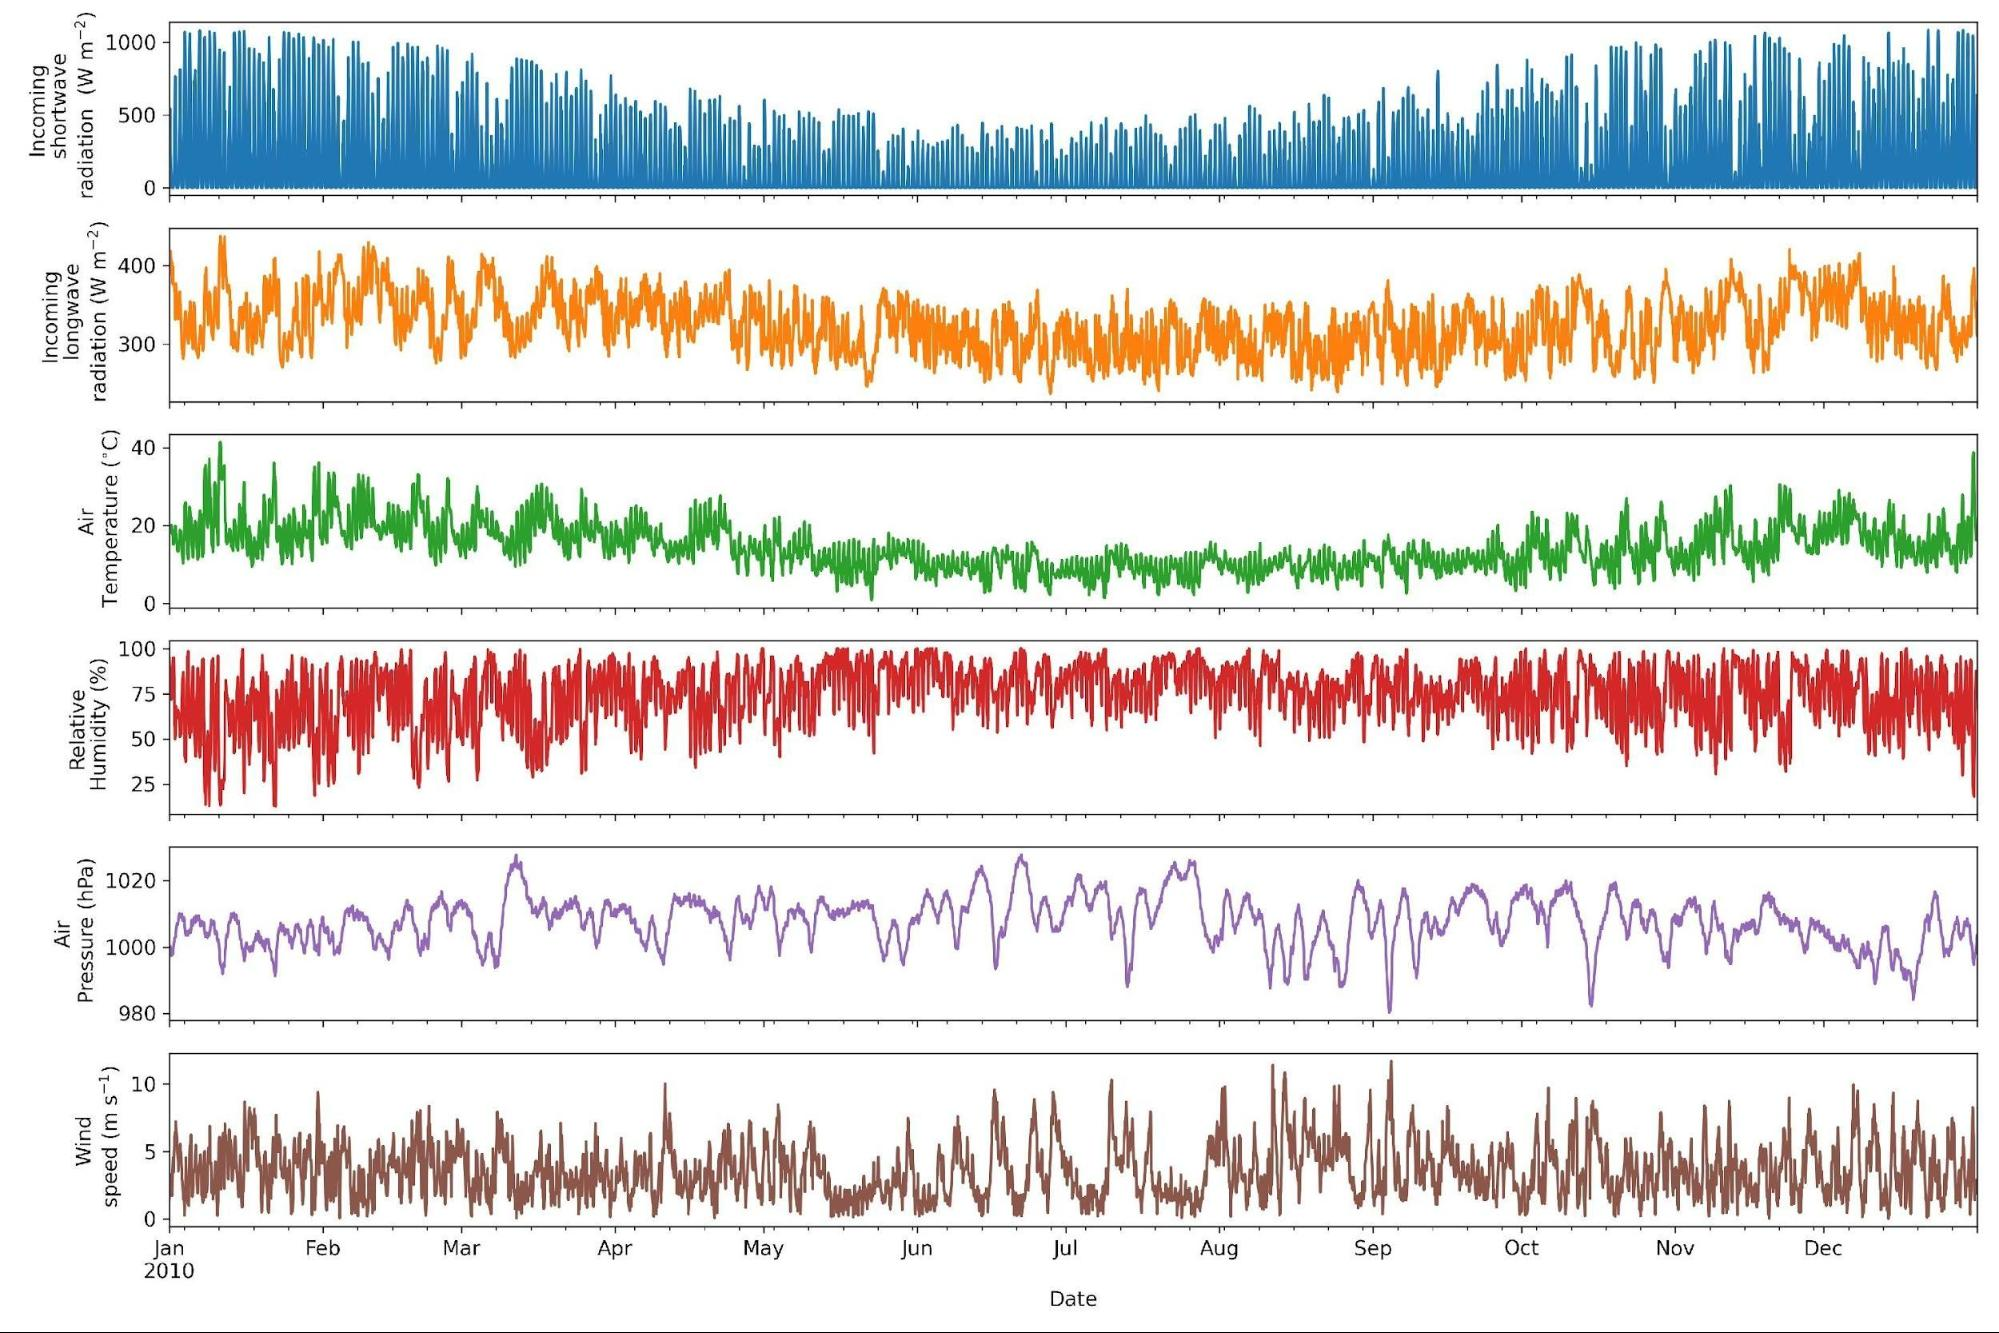
\includegraphics[trim={0 0 0 0},clip,scale=0.15]{images/image1.jpg}
\caption{\bf Historic hourly ERA5 forcing meteorology for Melbourne, showing only 2010 as an example.}
 \label{fig:mel_era5}
\end{figure}

Climate change data are taken from the most recent Coupled Model Intercomparison Project Phase 6 \citep{Eyring2016} (CMIP6) archive, developed within the framework of IPCC's 6th Assessment Report\citep{IPCC2021}. Since hourly output is typically not available from the global climate models (GCMs) available in CMIP6, daily minimum, mean and maximum temperature are extracted from 17 CMIP6 models, for:

\begin{itemize}
\item all nine capital cities and regional centres
	\item three shared socioeconomic pathways (SSP) emission scenarios:
	\begin{itemize}
	\item 1.2-6: Limit warming below 2$^{\circ}$C, 
	\item 3.7-0: Middle of the road -- current trajectory, 
	\item 5.8-5: No policy (worst-case) scenario
	\end{itemize}
\item two future periods: centred on 2030 and 2050
\end{itemize}

The air temperature climate change signal obtained from CMIP6 data is superimposed onto the historic ERA5 time series via a `morphing' process. This technique refers to the application of a shift (in mean) and a stretch (in minimum and maximum) of the observed time series, to change both the mean and the variance \citep{Belcher2005,Pulkkinen2021}. For each month, a minimum, median, and maximum air temperature change is computed as the ensemble median over all CMIP6 models, per city, SSP scenario, and future period (see Figure \ref{fig:MelCmip} for Melbourne example). 

\begin{figure}
\centering
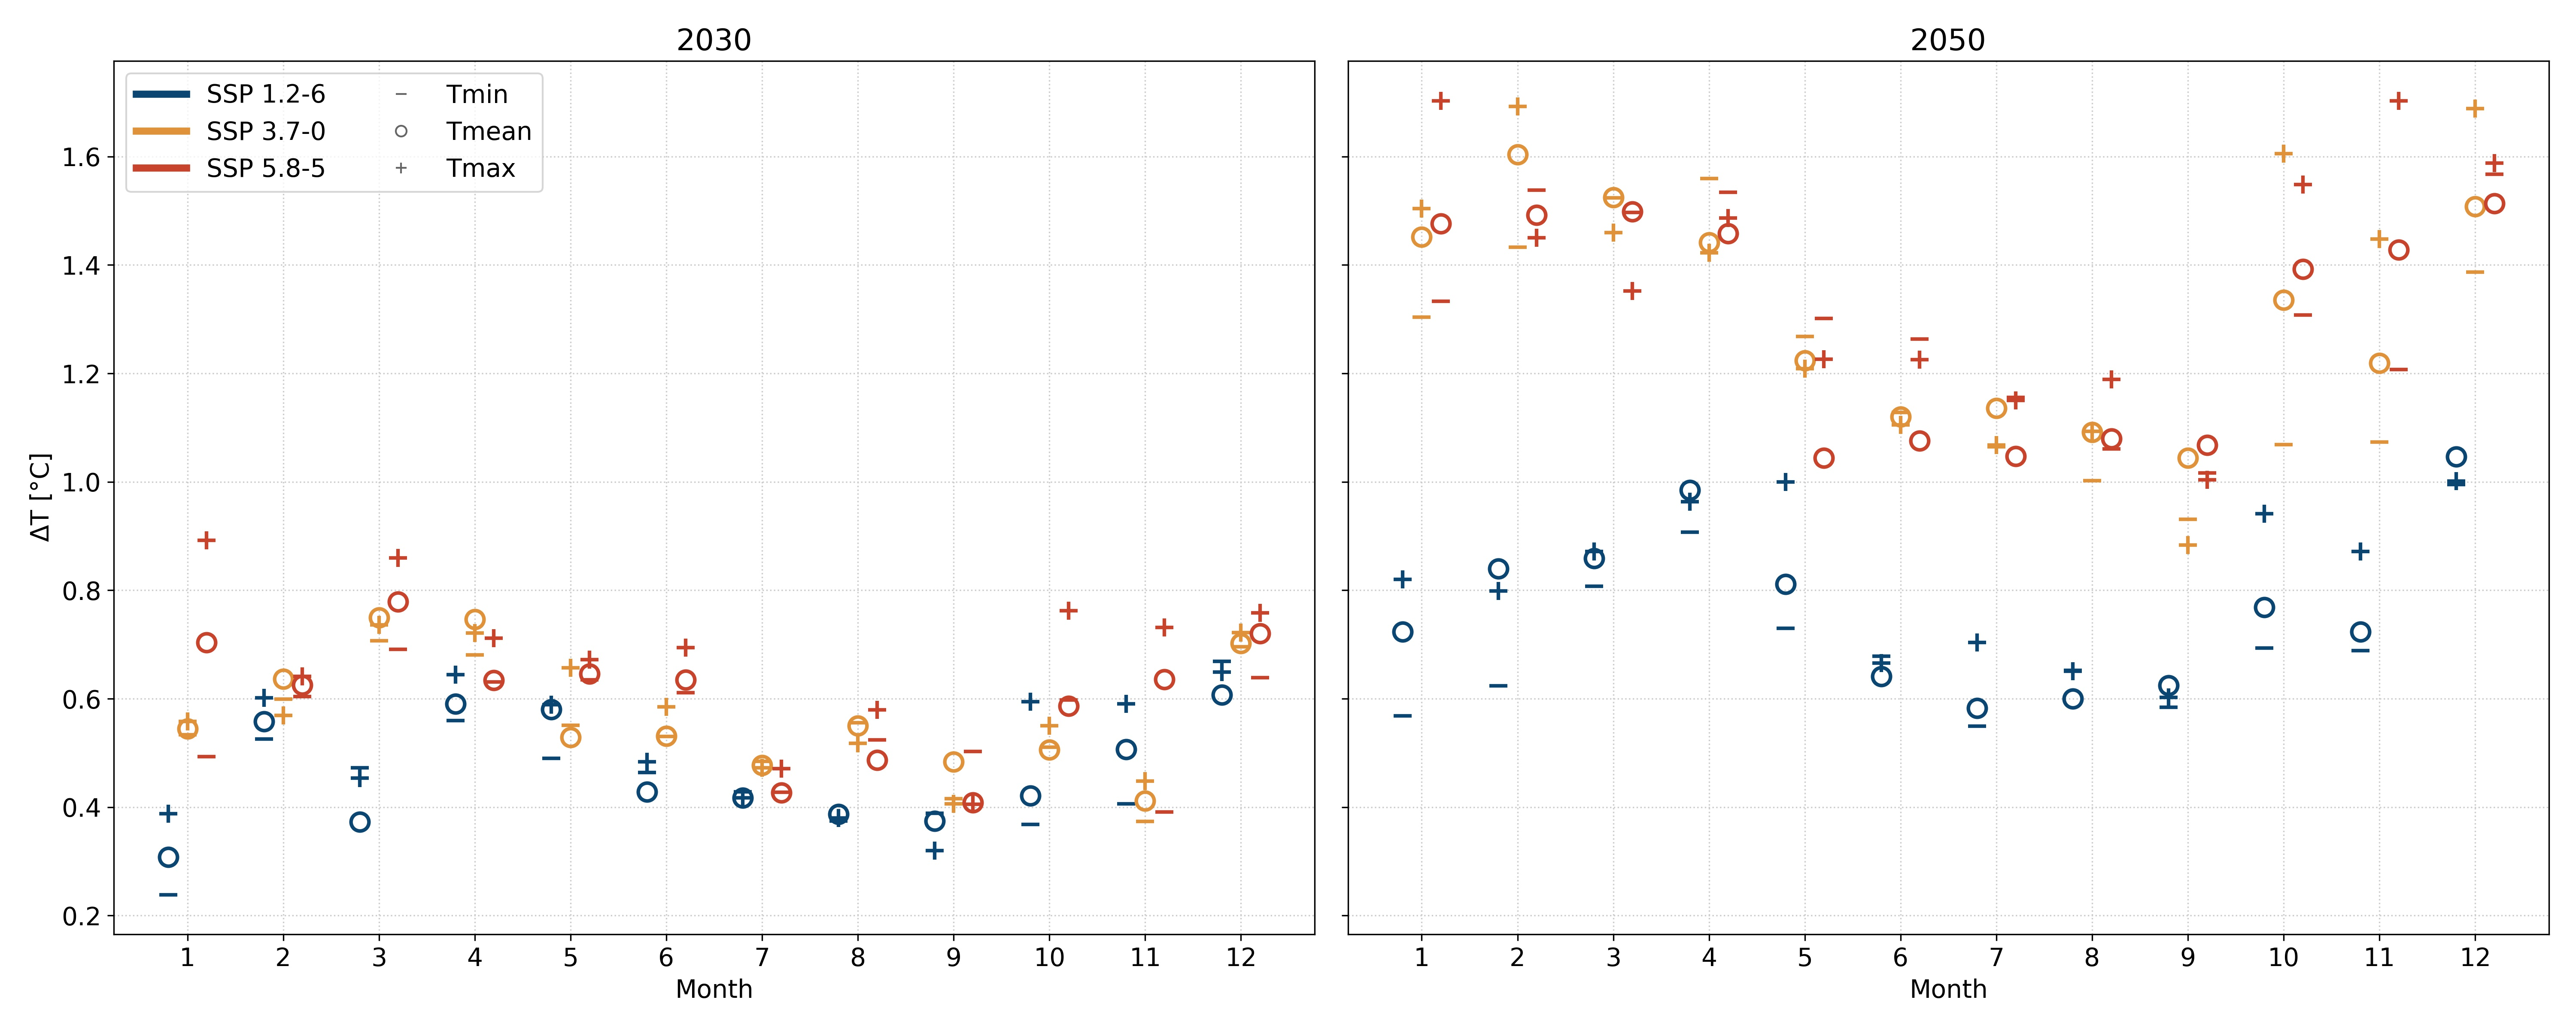
\includegraphics[trim={30 30 20 30},clip,scale=0.15]{images/image2.jpg}
\caption{\bf Projected minimum, mean and maximum monthly temperatures for Melbourne, changes ($\Delta$T, $^{\circ}$C), as the median over all 17 CMIP6 models, for SSPs 1.2-6, 3.7-0, 5.8-5, and target periods 2030 (left) and 2050 (right).}
 \label{fig:MelCmip}
\end{figure}

Superimposing the CMIP6 ensemble median monthly minimum, mean and maximum $\Delta$T onto the ERA5 historical air temperature provides a detailed yet nuanced new time series of projected future air temperatures (Figure \ref{fig:MelHist} for Melbourne).  The seasonal plots in Figure \ref{fig:MelHist} indicate that temperature changes are variable in time, with the strongest warming in summer months, and a more moderate warming in cooler months. Simultaneously, warming patterns are often asymmetric (e.g., the long right-hand tail of $\Delta$T for SSP 5.8-5 in SON 2050), indicating that extremes may become more pronounced in the future.
This procedure has been finalised for all nine capital cities and regional centres (not shown), which means that all meteorological and climate change information are available to run TARGET.

\begin{figure}
\centering
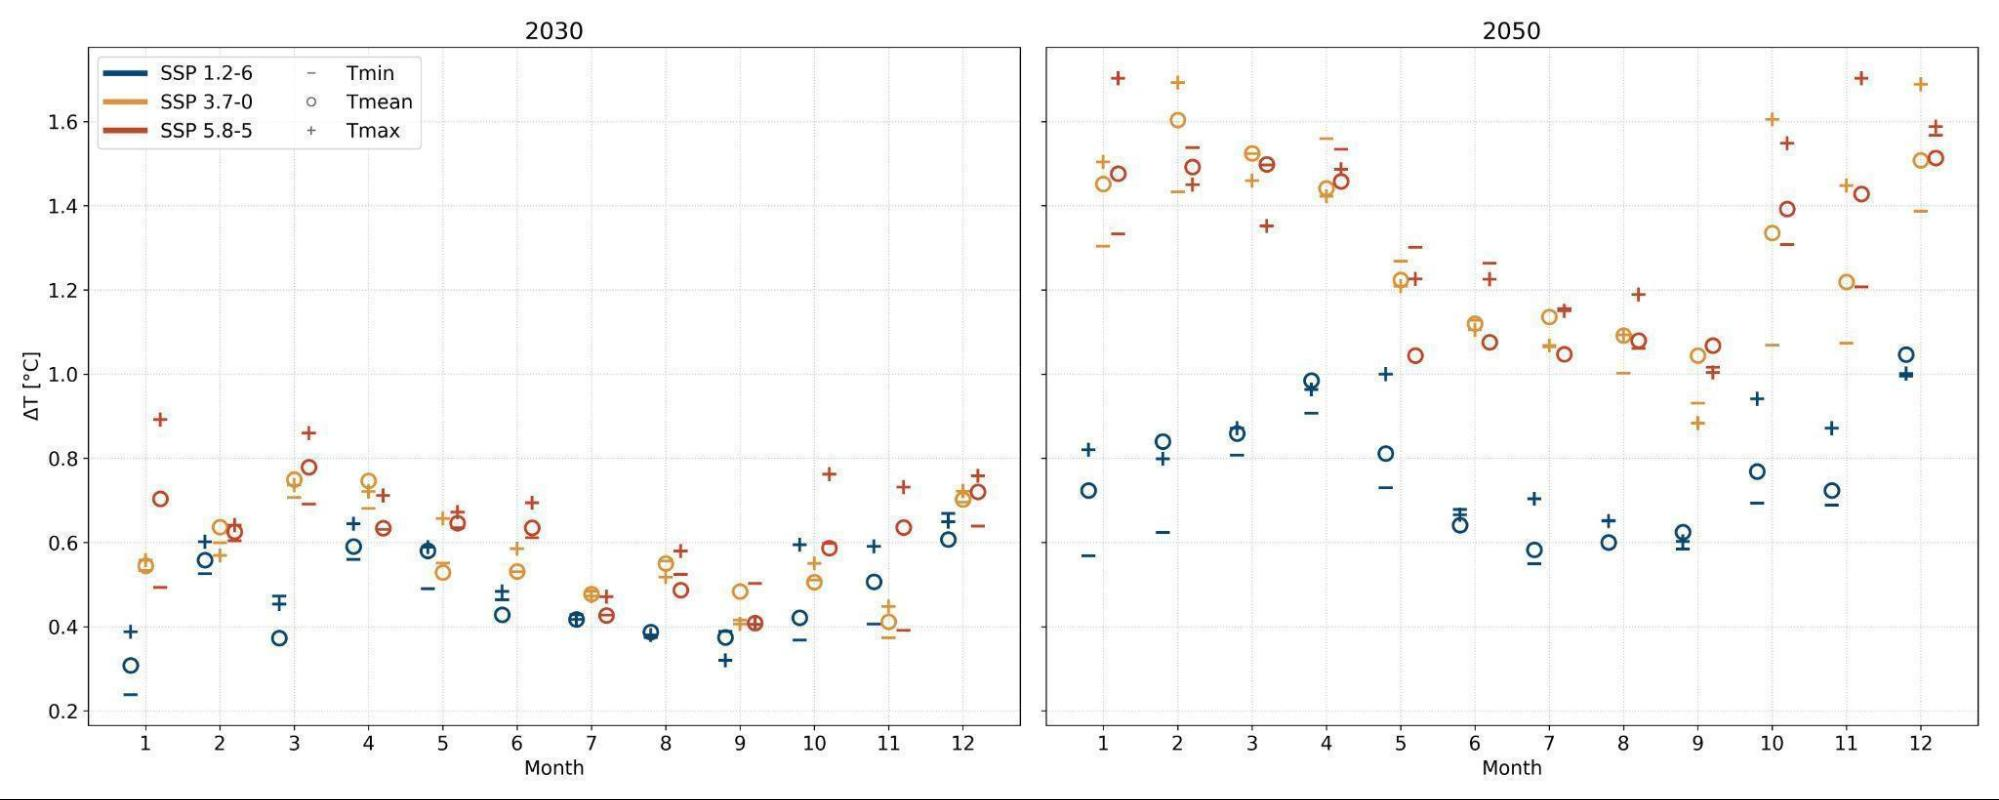
\includegraphics[trim={0 0 0 0},clip,scale=0.25]{images/image3.jpg}
\caption{\bf Seasonal histograms of hourly temperature change between the morphed future time series and the historical ERA5 time series, for Melbourne. Future time series reflect both the SSPs emission scenarios (line colours) and target future periods (line types). DFJ, MAM, JJA, and SON refer to the meteorological seasons: austral summer (December-January-February), autumn (March-April-May), winter (June-July-August), and spring (September-October-November).}
 \label{fig:MelHist}
\end{figure}

\subsection{Land cover fractions and IWM interventions}\label{sec:lc}

The land cover (fraction) for all nine selected cities is described using the LCZ typology \citep{Stewart2012b}. This is a holistic and global approach that allocates landscapes according to properties that influence screen-height temperature, namely surface structure (height and spacing of buildings and trees) and surface cover (pervious including vegetation, or impervious). As each of the 17 LCZ classes (10 of which are built LCZs, see \ref{sec:appendix1}.) are associated with key urban canopy parameters \citep{Ching2018a}, this scheme is extremely well-suited for providing universal and consistent land cover fraction data to 1) implement TARGET at the surface for a present-day scenario, and 2) devise IWM scenarios for use in TARGET. Here, the LCZ maps for all 9 cities are extracted from a global LCZ map available at a 100 m spatial resolution \citep{Demuzere2022}. The LCZ map for Melbourne is shown in Figure \ref{fig:MelLCZ} as an example.

\begin{figure}
\centering
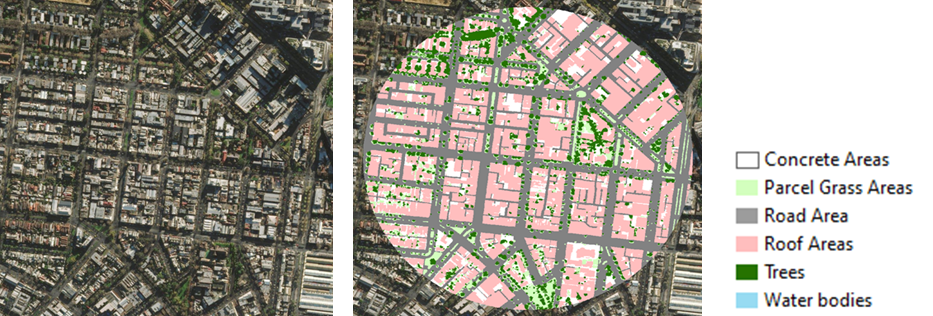
\includegraphics[trim={0 0 0 0},clip,scale=0.35]{images/image4.png}
\caption{\bf LCZ map for Melbourne.}
 \label{fig:MelLCZ}
\end{figure}

Each of the LCZ typologies are assigned geometric properties (e.g., ratio of building height to street width) and surface cover fractions (e.g., impervious surface fractions). \cite{Stewart2012b} provide a range of values from which default values can be derived. Within these ranges, we sought to assign more accurate geometric and surface cover fractions for the Australian context that better represent the urban form found in Australian cities. Using a combination of grid point identification and GIS Land Use Land Cover databases, surface cover fractions were derived for each LCZ for the current urban landscape (business as usual: BAU) as shown for LCZ2 as an example in Figure \ref{fig:surfCovFrac} and Table \ref{table:lcz2}.

\begin{figure}
\centering
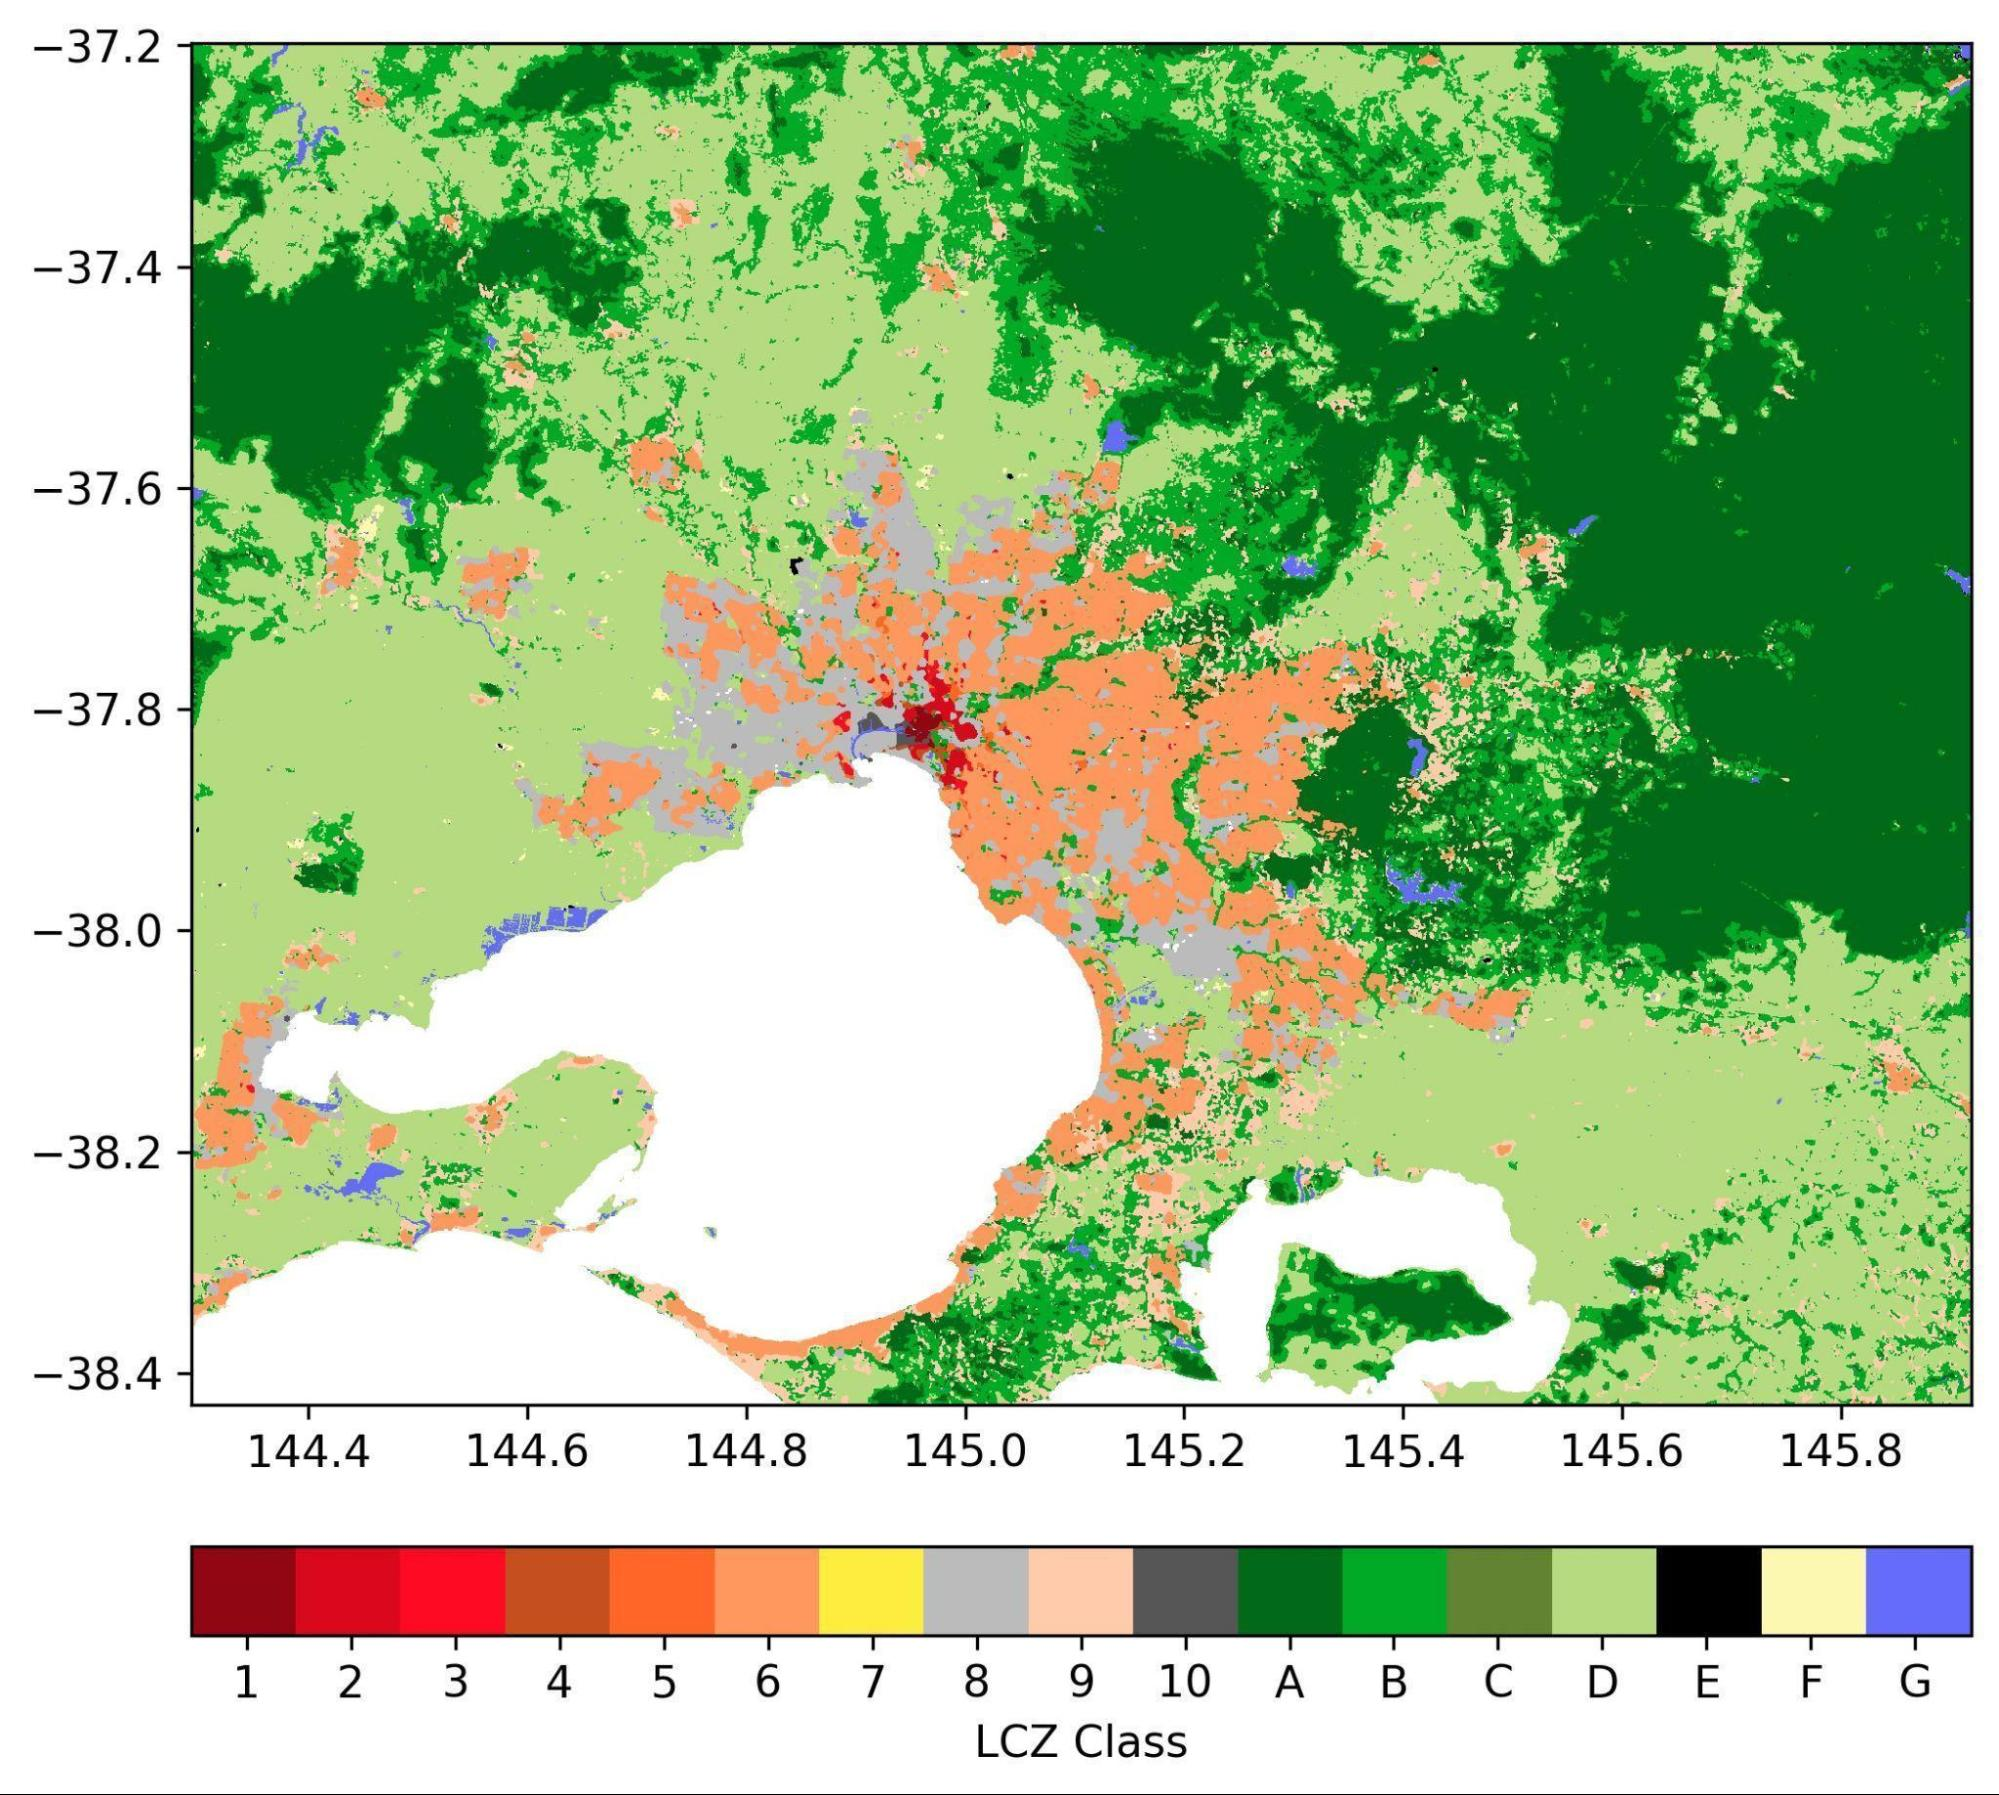
\includegraphics[trim={0 0 0 0},clip,scale=0.15]{images/image5.jpg}
\caption{\bf Example of the use of Land Use Land Cover maps to derive surface cover fractions.}
 \label{fig:surfCovFrac}
\end{figure}

\setlength\arrayrulewidth{1pt} %Increasing linewidth 
\begin{table}[!ht]
\caption{Example geometric properties (BH building height and VH vegetation height) and surface cover properties (A: fraction of surface type, and total impervious and pervious) for LCZ2. Subscripts to A refer to \textit{roof}, \textit{conc} (concrete), \textit{asph} (asphalt), \textit{grass}, \textit{igrs} (irrigated grass), \textit{tree}, \textit{water}, and \textit{imp} (impervious) and \textit{per} (pervious) surface and land cover types. BAU business as usual (current land cover), MOD = moderate IWM interventions, HIGH = High IWM interventions.}
    \centering
    \begin{tabular}{|l|l|l|l|l|l|l|l|l|l|l|l|}
    \hline
       \rowcolor{light-gray} LCZ2  & A$_{roof}$  & A$_{conc}$  & A$_{asph}$  & A$_{grass}$  & A$_{igrs}$  & A$_{tree}$  & A$_{water}$  & A$_{imp}$  & A$_{per}$  & BH  & VH  \\ \hline
        BAU & 52 & 6 & 24 & 4 & 2 & 12 & 0 & 82 & 18 & 15 & 8 \\ \hline
        MOD & 52 & 4 & 16 & 3 & 3 & 21 & 1 & 72 & 28 & 15 & 8 \\ \hline
        HIGH & 48 & 4 & 10 & 1.5 & 4 & 30 & 2.5 & 62 & 38 & 15 & 8 \\ \hline
    \end{tabular}\label{table:lcz2}
\end{table}
\setlength\arrayrulewidth{0.4pt} %Back to default

Based on the current LCZ typologies for BAU, new typologies were developed that reflect the implementation of IWM. The interventions to be explored here focus on increasing tree canopy cover, retention of water in the urban landscape through water sensitive urban design, and irrigation (active or passive), and an overall shift from impervious (concrete/asphalt), to pervious surfaces, where possible. Several Australian states, territories, and Local Government Areas (LGA) are developing strategies or design guidelines that aim to mitigate urban heat. For example, the Parramatta Heat Strategy \citep{Paramatta2021} aims to "Increase canopy cover to 40\% by 2050 (based on 2016 levels)." The Western Sydney Regional Organisation of Council's (WSROC) \citep{WSROC2021} Turn Down the Heat Strategy and Action Plan aims to "Reduce the average peak ambient temperatures in Western Sydney by 1.5$^{\circ}$C through water, greening and cool materials strategies by 2023." The draft NSW State Environmental Planning Policy (Design and Place) 2021 (SEPP) \citep{NewSouthWales2021} includes a design consideration for green infrastructure including "whether the development maximises tree canopy cover and provides sufficient deep soil to support the tree canopy."

To develop future scenarios of IWM for implementation in this study, quite specific information is needed rather than broad guidelines that are more usually available in strategic reports. The NSW Government draft Urban Design Guide (2021) \citep{NewSouthWales2021} provides canopy cover targets for street trees and lots across different urban land use types. The NSW Government Apartment Design Guide (2015) \citep{NSW2015} specifies `deep soil zone' targets expected to support vegetation. The tree canopy cover and deep soil zone targets proposed in these guides align with the scenarios developed for each of the LCZ typologies (Table \ref{table:canopytargets}). In addition, for the ACT, Canberra's Living Infrastructure Plan: Cooling the City \citep{ACTGovernment2019}, a goal of 30\% permeable surfaces by 2045 has been set, along with a goal of 30\% tree canopy cover, and the Port Phillip Council in Melbourne requires that at least 20\% of surfaces must be permeable \citep{CityofPortPhillip2018}.

\setlength\arrayrulewidth{1pt} %Increasing linewidth 
\begin{table}[!ht]\caption{Tree canopy targets. The table shows BAU surface cover fractions (BAU) followed by tree canopy targets proposed in the NSW Draft Urban Design Guidelines. Targets are given for both street trees and lots in various development categories.}
    \centering
    \begin{tabular}{|p{0.85cm}|l|p{4.25cm}|l|p{3.75cm}|l|l|l|}
    \hline
         \rowcolor{dark-blue}  &BAU   & Street tree canopy   & Target\tablefootnote{\label{targets}Targets for streets with overhead power lines}   & Development category & Target   & MOD   &    \\ \hline
        \rowcolor{light-blue!25} LCZ1  & 8\% & Business parks & 35\% & Business parks (min deep soil target) & 7\%\tablefootnote{Target for min deep soil zone in the Apartment Design Guide} & 14\% & 20\% \\ \hline
        \rowcolor{light-gray} LCZ2 & 12\% & Existing residential streets (12-20 m reserve) & 40\% & Apartments (deep soil target) & 15\%\tablefootnote{Target for deep soil zone for lots sizes $>$1500m$^{2}$ in the Apartment Design Guide} & 21\% & 30\% \\ \hline
        LCZ3 \cellcolor{light-blue!25} & ~\cellcolor{light-gray} & ~\cellcolor{light-gray} & ~\cellcolor{light-gray} & ~\cellcolor{light-gray} & ~\cellcolor{light-gray} & ~\cellcolor{light-gray} & ~\cellcolor{light-gray} \\ \hline       
        \rowcolor{light-gray} LCZ4 & 10\% & ~ & ~  & Attached dwellings (150-300 m$^{2}$ lot size) & 20\% & 20\% & 30\%  \\ \hline
        LCZ5 \cellcolor{light-blue!25} & ~\cellcolor{light-gray} & ~\cellcolor{light-gray} & ~\cellcolor{light-gray} & ~\cellcolor{light-gray} & ~\cellcolor{light-gray} & ~\cellcolor{light-gray} & ~\cellcolor{light-gray} \\ \hline
        \rowcolor{light-gray} LCZ6 & 19\% & ~ & ~ & Detached dwellings (300-600 m$^{2}$ lot size) & 25\% & 27\% & 35\%  \\ \hline
        \rowcolor{light-blue!25} LCZ8 & 4\% & Existing industrial streets (20-25 m reserve) & 35\% & Industrial & 25\% & 14\% & 25\% \\ \hline
        LCZ10 \cellcolor{light-gray}& ~\cellcolor{light-blue!25} & ~\cellcolor{light-blue!25} & ~\cellcolor{light-blue!25} & ~\cellcolor{light-blue!25} & ~\cellcolor{light-blue!25} & ~\cellcolor{light-blue!25} & ~\cellcolor{light-blue!25} \\ \hline
        \rowcolor{light-blue!25} LCZ9\tablefootnote{LCZ9 is `sparsely built'. While the targets here apply, there is minimal street and development coverage in this LCZ.} & 17\% & Existing residential streets (12-20 m reserve) & 40\% & Detached dwellings ($>$600 m$^{2}$ lot size) & 35\% & 21\% & 25\% \\ \hline
        \rowcolor{light-gray} LCZB & 50\% & Public open space & 45\% & ~ & ~ & 50\% & 50\% \\ \hline
        LCZD \cellcolor{light-blue!25}& 50\% \cellcolor{light-blue!25}& ~\cellcolor{light-gray} & ~\cellcolor{light-gray} & ~\cellcolor{light-gray} & ~\cellcolor{light-gray} & ~\cellcolor{light-gray} & ~\cellcolor{light-gray} \\ \hline
    \end{tabular}\label{table:canopytargets}
\end{table}
\setlength\arrayrulewidth{0.4pt} %Back to default

IWM includes water sensitive urban design features such as rainwater tanks, raingardens, tree-pits, swales, and wetlands, as well as alternative water sources for irrigation. In TARGET, these features are represented by the surface type `irrigated grass' and water bodies. In planning documents for IWM strategy there is almost no specification of targets for each of the interventions and there is little alignment between individual jurisdictions.  

To develop a consistent approach across all the cities and LCZ typologies in this study two of our team members, with a combined 20 years working in the IWM/WSUD field, developed the `moderate' and `high' IWM scenarios for each of the LCZs. These were developed to be broadly consistent with the guidelines available (e.g., see above and Table \ref{table:canopytargets}) along with professional judgement of what might reasonably be accomplished. 

An iterative process was employed so that the total area of pervious and impervious surface summed to 100\% of the LCZ (see Table \ref{table:lcz2}).  Figure \ref{fig:surflcz} shows the finalised moderate and high IWM interventions for all LCZ classes used in this study.

\begin{figure}
\centering
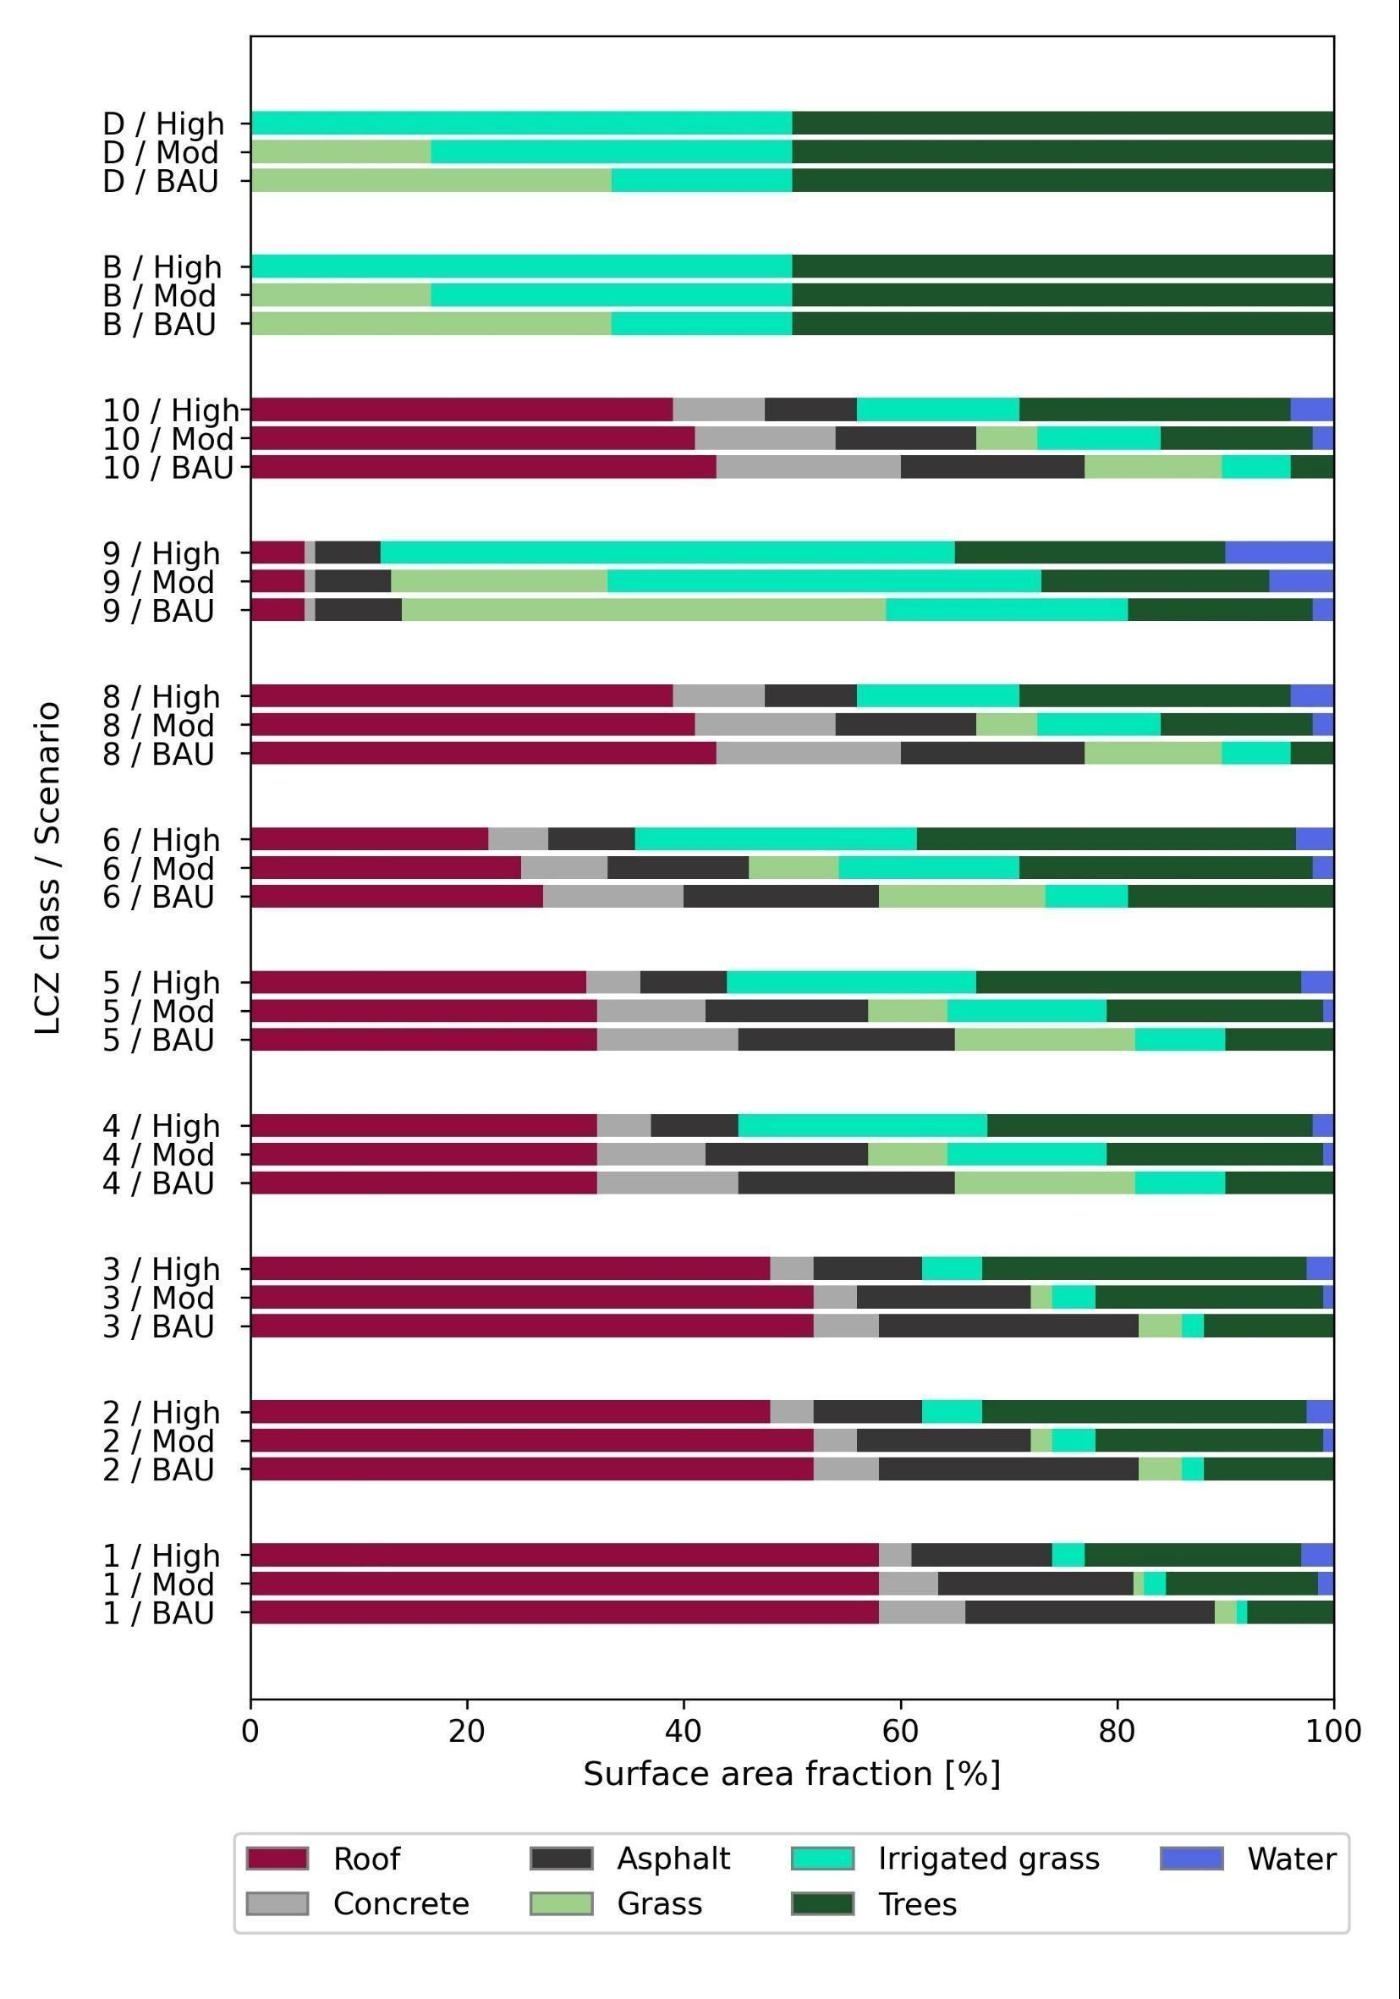
\includegraphics[trim={0 0 0 0},clip,scale=0.20]{images/image7.jpg}
\caption{\bf Surface cover fractions of each LCZ for BAU, moderate IWM interventions and high IWM interventions.}
 \label{fig:surflcz}
\end{figure}

To account for tropical/subtropical cities with pronounced wet seasons (Darwin, Townsville, and Brisbane) a dry season / wet season `switch', based on the local rainfall climatology, was applied to each of those cities so that effectively these landscapes were fully "irrigated" during their wet season. This was because the "unirrigated" vegetation did not reflect the substantial moisture associated with those areas during the wet summer months for the TARGET modelling on the largely naturally vegetated LCZs 9, B and D. The dates for the switch for dry seasons are May 1 - November 1 for Darwin, April 1 - January 1 for Townsville and August 1 - December 1 for Brisbane. 

\subsection{Spatial aggregation of LCZs to SA4 areas and entire cities}

For this project the health outcomes data were requested for the Australian cities at Statistical Area Level 4 (SA4s). These are geographic areas built from whole Statistical Areas Level 3 (SA3s) and are the largest sub-state regions in the Main Structure of the ASGS (Australian Statistical Geography Standard). They are designed for the output of a variety of regional data, including the 2021 Census data. For this reason, all LCZ and TARGET outputs for each city have been mapped onto the local SA4 areas. However, for many cities the SA4 areas include large areas (often $>$50\%) of rural and natural landscape that have little population and no IWM interventions. The presence of these areas' "washes" out the IWM benefits when averaged across the whole SA4 area, so we needed to find a valid way of removing this effect. The approach used is described below.

For each city, only the urban fraction of the SA4 statistical areas is selected, using the global urban boundaries database (GUB) from \cite{Li2020b}. The LCZ map is then extracted for each SA4-GUB intersection, and the relative LCZ class weights are calculated (considering all built LCZs (1 to 10) and LCZs B and D). Finally, these weights are used to calculate the TARGET temperatures representative for the urban fraction of the SA4 sector. Figure \ref{fig:sa4maps} provides an example of the process for Adelaide. The weighted SA4 areas can then be aggregated again to generate a city-wide value of the temperature metric required (air temperature or amount of cooling observed, etc.).

\begin{figure}
\centering
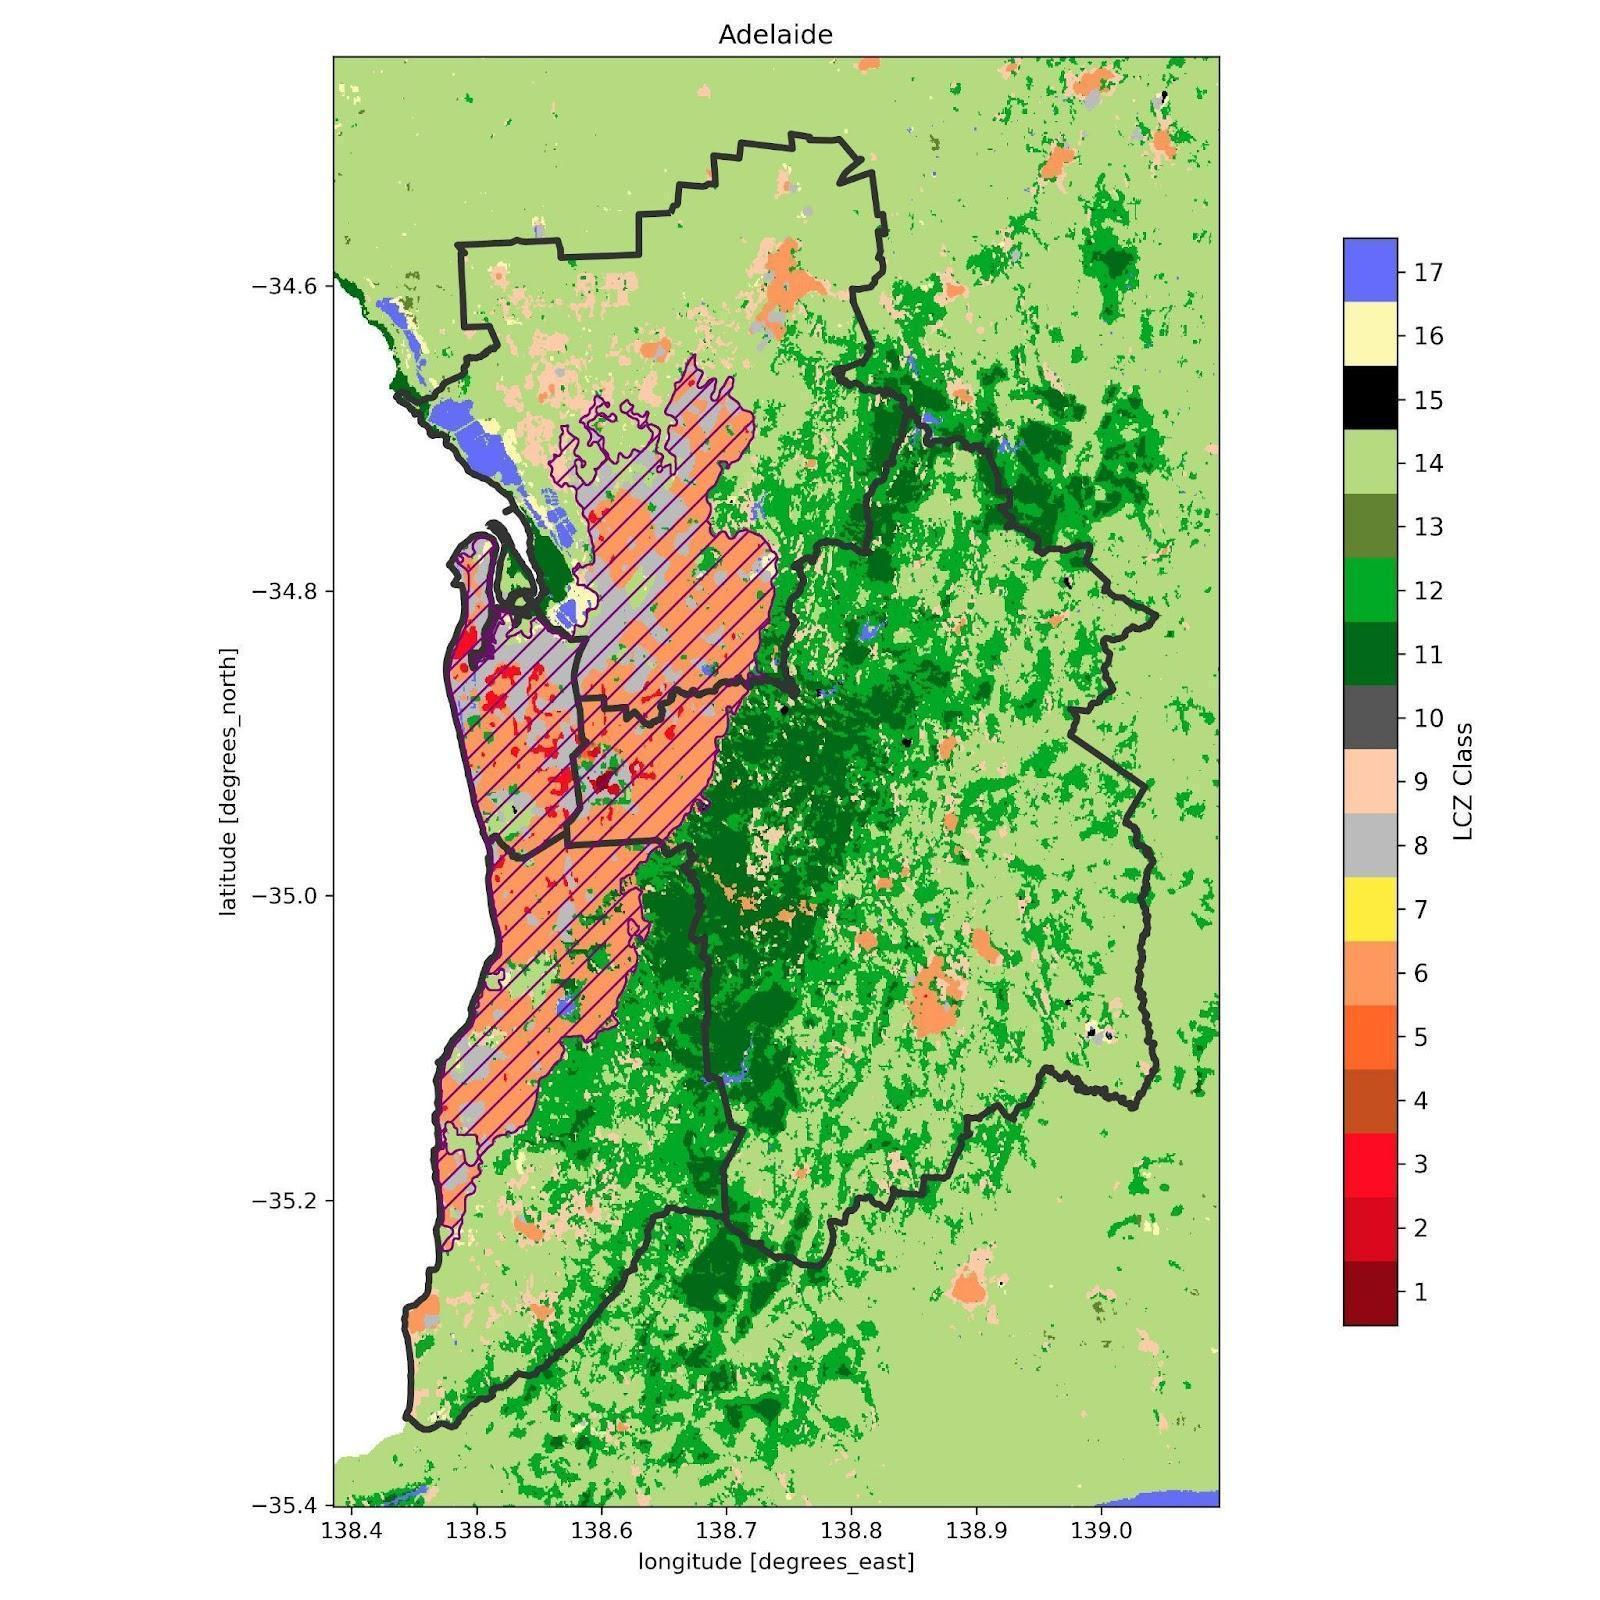
\includegraphics[trim={0 0 0 0},clip,scale=0.25]{images/image6.jpg}
\caption{\bf Mapping the SA4 areas from the LCZ areas and the GUB.  The LCZ areas for Adelaide are shown. The black lines show the SA4 statistical areas that intersect with the GUB urban boundary (purple). The purple hatched areas indicate the parts of the SA4 sections that are used to derive the LCZ class weights.}
 \label{fig:sa4maps}
\end{figure}

\section{Results}\label{sec:results}
\subsection{Results of TARGET modelling for all cities}\label{sec:results1}

Scenario modelling was performed for all LCZ classes and their IWM variations (BAU, MODERATE, HIGH) for all cities using ERA5 2010-2020 present day climate conditions as well as CMIP6-adjusted 2030 and 2050 SSP 1.2-6, 3.7-0, and 5.8-5 future climate scenarios. 

The climate modelling for this project has produced a vast amount of data.  The complete data set is available at (INSERT LOCATION) with tables summarising the full set of results for each of the nine Australian cities are provided in \ref{sec:appendix2}. The key points arising from examining these data are summarised below. The summary data are average daily values for 10-year time periods centred on 2015 (historical data), 2030, and 2050. Cooling for all cities associated with implementation of IWM is calculated as moderate [MOD] or high [HIGH] minus business as usual [BAU] temperatures.

\subsubsection{Spatial variation in temperature across cities}\label{sec:results1a}

The climate of cities depends on their geographical location, local meteorology, and the form of the urban environment. It is well known that more built up areas are generally warmer than less built up and rural areas, particularly at night. However, because this is a relative comparison, these patterns do depend on the type, and moisture status, of natural surfaces. Data was collated at the SA4 level. For smaller cities (e.g., Canberra and Darwin) the SA4 level data covers the entire urban area. For larger cities, such as Melbourne and Sydney, there are several SA4s meaning spatial variability in temperature can be seen. It should be noted though, that the outer SA4s do extend beyond the boundary of urban development and vary with elevation and natural surface cover.

During the day, the SA4 that encompasses the CBD tends to be cooler than the surrounding low-density areas. Shading and heat storage during the day can lead to cooler temperatures in highly built-up areas. IWM tends to be more beneficial in low to medium density areas during the day. This is seen in both Brisbane and Melbourne (Figure \ref{fig:lczsa4}). At night, the central, high-density areas of the city are warmest due heat trapping by buildings and the slow release of stored energy from urban surfaces. 

\begin{figure}
\centering
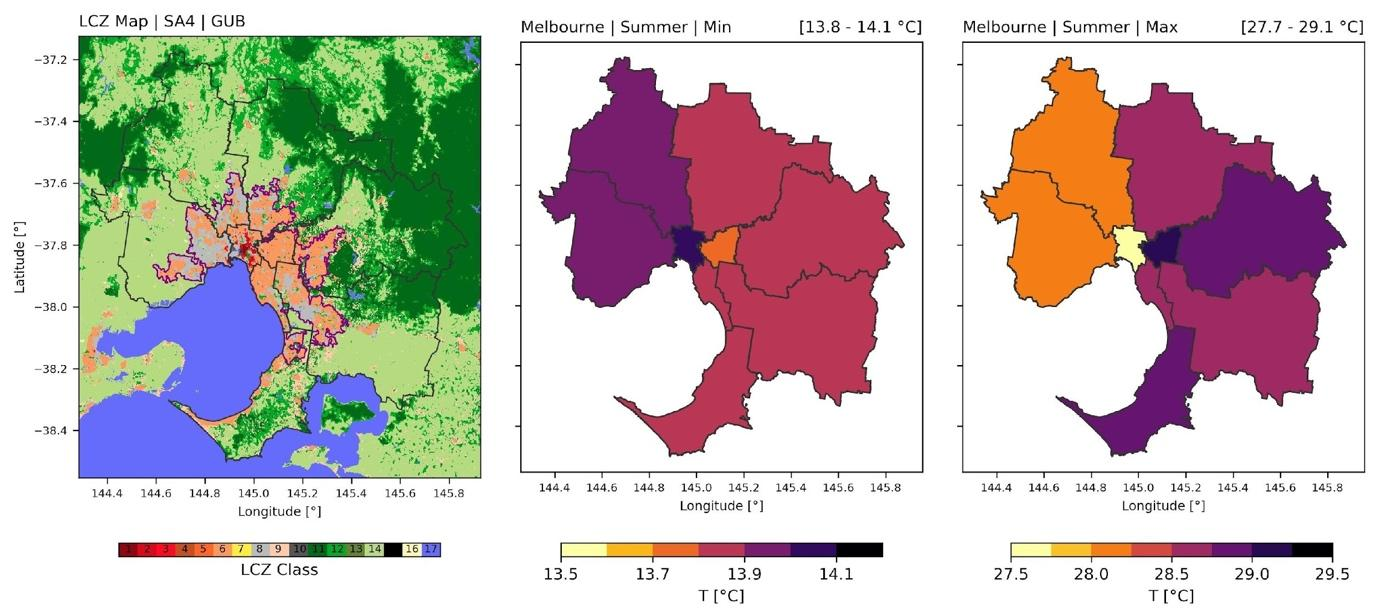
\includegraphics[trim={0 0 0 0},clip,scale=0.25]{images/image9.jpg}
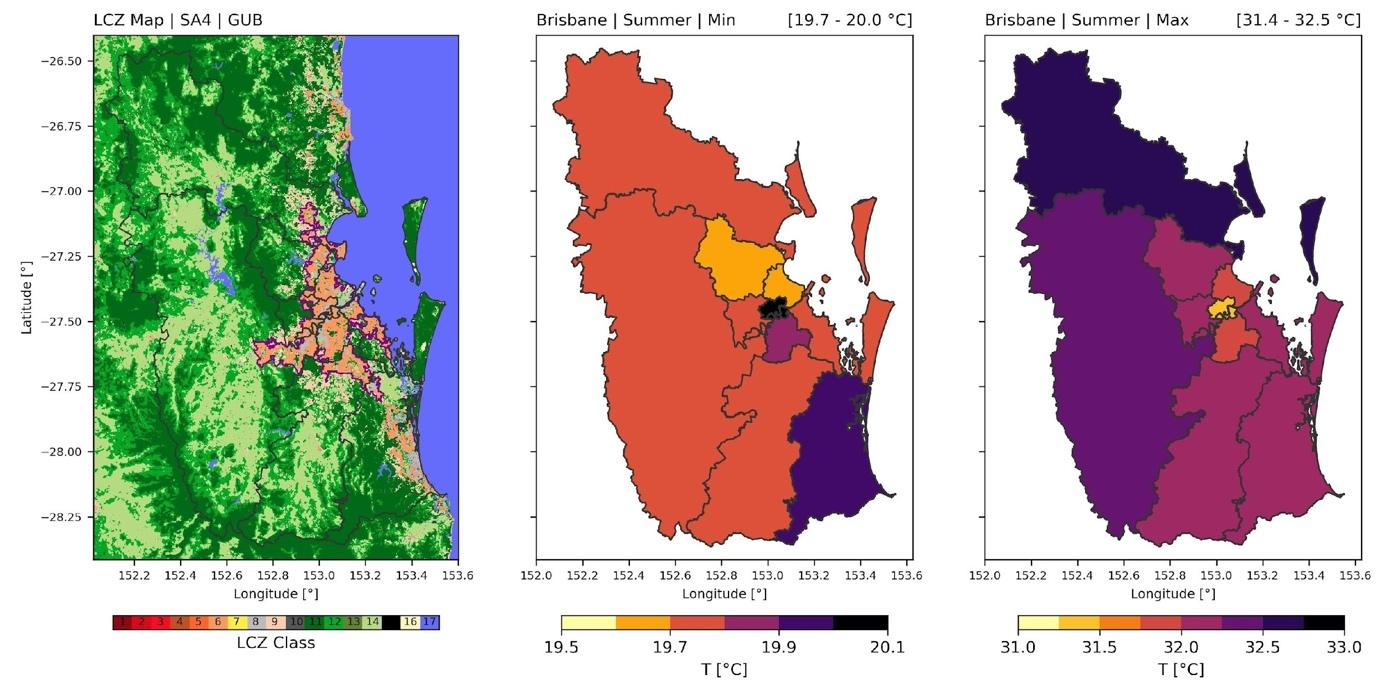
\includegraphics[trim={0 0 0 0},clip,scale=0.25]{images/image8.jpg}
\caption{\bf Present day LCZ map (left column), with SA4 (grey) and GUB (purple) boundaries. The middle and right panels indicate the (BAU) mean summer daily minimum (Min) and maximum (Max) temperatures respectively, for Melbourne (top row) and Brisbane (bottom row). Values in square brackets indicate the air temperature range across the available SA4 sections}
 \label{fig:lczsa4}
\end{figure}

\subsection{Impact of IWM on present day climate (BAU)}\label{sec:results2}

\subsubsection{Annual impact of IWM interventions}\label{sec:results2a}

The implementation of IWM for the present-day climate (as applied in TARGET) led to annual mean daily temperature reductions across all capital and regional cities. Results showed annual mean daily temperature reductions ranging from of -0.09$^{\circ}$C in Brisbane to -0.22$^{\circ}$C in Albury for MOD IWM interventions, and from -0.12$^{\circ}$C in Brisbane to -0.35$^{\circ}$C for HIGH IWM interventions (Table \ref{table:annual}). 

\setlength\arrayrulewidth{1pt} %Increasing linewidth 
\begin{table}[!ht]\caption{Present day (BAU) mean annual daily, maximum (max) and minimum (min) temperatures for each capital or regional city, and the associated temperature changes resulting from moderate (MOD) and high (HIGH) IWM interventions.}
    \centering
    \begin{tabular}{|p{1.5cm}|p{2.5cm}|p{1.0cm}|p{1.0cm}|p{1.0cm}|p{1.0cm}|p{1.0cm}|p{1.0cm}|p{1.0cm}|p{1.0cm}|}
    \hline
        \rowcolor{dark-blue}~ &Annual (mean daily) temperature &  ~ & ~ & ~ & ~ & ~ & ~ & ~ & ~ \\ 
        \rowcolor{dark-blue}City & BAU mean & BAU max & BAU   min & MOD       mean & MOD       max & MOD        min & HIGH      mean & HIGH      max & HIGH        min \\ \hline
        \rowcolor{light-gray}Adelaide & 15.81 & 24.03 & 9.56 & -0.19 & -0.97 & 0.3 & -0.31 & -1.67 & 0.55 \\ \hline
        \rowcolor{light-blue!25}Albury & 14.86 & 23.37 & 8.28 & -0.22 & -1.05 & 0.24 & -0.35 & -1.78 & 0.45 \\ \hline
        \rowcolor{light-gray}Brisbane & 19.86 & 26.91 & 14.49 & -0.09 & -0.56 & 0.15 & -0.12 & -0.86 & 0.28 \\ \hline
        \rowcolor{light-blue!25}Canberra & 12.64 & 21.23 & 6.22 & -0.18 & -0.96 & 0.23 & -0.29 & -1.63 & 0.42 \\ \hline
        \rowcolor{light-gray}Darwin & 27.33 & 33.99 & 22.39 & -0.12 & -0.51 & 0.08 & -0.18 & -0.77 & 0.14 \\ \hline
        \rowcolor{light-blue!25}Melbourne & 14.34 & 20.79 & 9.29 & -0.14 & -0.82 & 0.28 & -0.21 & -1.43 & 0.51 \\ \hline
        \rowcolor{light-gray}Perth & 17.41 & 26.46 & 10.86 & -0.15 & -1.05 & 0.43 & -0.25 & -1.86 & 0.8 \\ \hline
        \rowcolor{light-blue!25}Sydney & 17.01 & 25.49 & 10.83 & -0.14 & -0.89 & 0.24 & -0.22 & -1.49 & 0.45 \\ \hline
        \rowcolor{light-gray}Townsville & 23.54 & 29.46 & 18.89 & -0.11 & -0.41 & 0.07 & -0.17 & -0.62 & 0.12 \\ \hline
    \end{tabular}\label{table:annual}
\end{table}
\setlength\arrayrulewidth{0.4pt} %Back to default

We also considered the impact of IWM on annual mean maximum and minimum daily temperatures to identify the impact throughout the day. Results showed that the MOD IWM interventions reduced annual mean daily maximum temperatures from -0.51$^{\circ}$C in Darwin to -1.05$^{\circ}$C in Albury and Perth. The effect is even more pronounced for HIGH IWM interventions, with temperature reductions in annual mean daily maximum temperature ranging from -0.77$^{\circ}$C in Darwin, up to -1.86$^{\circ}$C in Perth (Table \ref{table:annual}).

The cooling behaviours described above are in line with expectations and are driven by the physical processes operating. MOD and HIGH IWM interventions provide increasing amounts of vegetation, shading and water availability compared with BAU. Evapotranspiration is maximised for abundant vegetation with a good water supply and is an extremely effective cooling mechanism, especially when the ambient air is dry and hot. 

Generally, the drier southern cities produce the greatest thermal response to implementation of IWM. Therefore, cities such as Perth, Albury and Adelaide show the largest reductions in annual mean maximum daily temperatures from IWM interventions, while cities of Melbourne, Canberra and Sydney show slightly lower reductions. In contrast, tropical cities, with pronounced wet seasons, produce the smallest thermal response as cooling associated with evapotranspiration is dramatically reduced when the ambient air is moist. This means reductions in annual mean maximum daily temperature from IWM interventions were smaller for Brisbane, Darwin, and Townsville (Table \ref{table:annual}). 

While the annual mean and maximum daily temperatures show reductions following the implantation of IWM, the annual minimum daily temperatures show an increase across all capital and regional cities. These increases range from 0.08$^{\circ}$C in Darwin, to 0.43$^{\circ}$C in Perth for the MOD interventions of IWM, and from 0.14$^{\circ}$C to 0.8$^{\circ}$C for the HIGH IWM interventions for Darwin and Perth respectively. The warming effect of IWM at times of minimum overnight temperature is also in line with expectations and is driven largely by increased storage of daytime heat in the soil (water dramatically increases soil thermal conductivity) followed by its nocturnal release. Cities that showed larger annual maximum daily temperature reductions from IWM also show larger increases in corresponding minimum temperatures. The degree of warming at the time of minimum temperature was unexpected and suggests that IWM could potentially provide health benefits at both ends of the temperature spectrum. This should be investigated further.

\subsubsection{Seasonal impact of IWM interventions}\label{sec:results2b}

The BAU mean daily, maximum, and minimum temperatures are also provided for Summer (DJF: Dec, Jan, Feb) in Table \ref{table:djf} and Winter (JJA: Jun, Jul, Aug) in Table \ref{table:jja}. Results showed that the cooling benefit of IWM is substantially enhanced during summer for most cities, but especially for the drier southern cities (Table \ref{table:djf}). This is most evident in the mean maximum daily temperatures, meaning IWM interventions (especially if implemented widely as in the HIGH case) can help reduce the heat exposure.

\setlength\arrayrulewidth{1pt} %Increasing linewidth 
\begin{table}[!ht]\caption{Present day (BAU) mean austral summer (DJF) daily, maximum (max) and minimum (min) temperatures for each capital or regional city, and the associated temperature changes resulting from moderate (MOD) and high (HIGH) IWM interventions.}
    \centering
    \begin{tabular}{|p{1.5cm}|p{2.5cm}|p{1.0cm}|p{1.0cm}|p{1.0cm}|p{1.0cm}|p{1.0cm}|p{1.0cm}|p{1.0cm}|p{1.0cm}|}
    \hline
        \rowcolor{dark-blue}~ &Austral summer DJF (average daily) &  ~ & ~ & ~ & ~ & ~ & ~ & ~ & ~ \\ 
        \rowcolor{dark-blue}City & BAU mean & BAU max & BAU   min & MOD       mean & MOD       max & MOD        min & HIGH      mean & HIGH      max & HIGH        min \\ \hline    
		\rowcolor{light-gray}Adelaide & 23.12 & 33.67 & 14.77 & -0.62 & -1.67 & 0.12 & -1.1 & -2.91 & 0.22 \\ \hline
        \rowcolor{light-blue!25}Albury & 23.92 & 34.97 & 15.31 & -0.71 & -1.91 & 0.07 & -1.25 & -3.32 & 0.14 \\ \hline
        \rowcolor{light-gray}Brisbane & 24.99 & 32.03 & 19.77 & -0.27 & -0.77 & 0.08 & -0.43 & -1.21 & 0.16 \\ \hline
        \rowcolor{light-blue!25}Canberra & 20.72 & 31.22 & 12.79 & -0.6 & -1.68 & 0.09 & -1.05 & -2.88 & 0.18 \\ \hline
        \rowcolor{light-gray}Darwin & 28.24 & 33.56 & 24.64 & -0.13 & -0.49 & 0.1 & -0.19 & -0.77 & 0.19 \\ \hline
        \rowcolor{light-blue!25}Melbourne & 20.43 & 28.42 & 13.91 & -0.57 & -1.42 & 0.05 & -1 & -2.53 & 0.11 \\ \hline
        \rowcolor{light-gray}Perth & 24.52 & 36.03 & 16.08 & -0.58 & -1.74 & 0.23 & -1.04 & -3.12 & 0.42 \\ \hline
        \rowcolor{light-blue!25}Sydney & 23.49 & 32.78 & 16.83 & -0.43 & -1.35 & 0.13 & -0.74 & -2.32 & 0.27 \\ \hline
        \rowcolor{light-gray}Townsville & 27.45 & 33.28 & 23.03 & -0.22 & -0.59 & 0.07 & -0.35 & -0.93 & 0.14 \\ \hline
    \end{tabular}\label{table:djf}
\end{table}
\setlength\arrayrulewidth{0.4pt} %Back to default

\setlength\arrayrulewidth{1pt} %Increasing linewidth 
\begin{table}[!ht]\caption{Present day (BAU) mean Austral winter (JJA) daily, maximum (max) and minimum (min) temperatures for each capital or regional city, and the associated temperature changes resulting from moderate (MOD) and high (HIGH) IWM interventions.}
    \centering
    \begin{tabular}{|p{1.5cm}|p{2.5cm}|p{1.0cm}|p{1.0cm}|p{1.0cm}|p{1.0cm}|p{1.0cm}|p{1.0cm}|p{1.0cm}|p{1.0cm}|}
    \hline
        \rowcolor{dark-blue}~ &Austral summer JJA (average daily) &  ~ & ~ & ~ & ~ & ~ & ~ & ~ & ~ \\ 
        \rowcolor{dark-blue}City & BAU mean & BAU max & BAU   min & MOD       mean & MOD       max & MOD        min & HIGH      mean & HIGH      max & HIGH        min \\ \hline    
        \rowcolor{light-gray}Adelaide & 8.86 & 14.83 & 4.57 & 0.2 & -0.33 & 0.51 & 0.41 & -0.54 & 0.92 \\ \hline
        \rowcolor{light-blue!25}Albury & 6.47 & 12.51 & 1.92 & 0.19 & -0.25 & 0.4 & 0.39 & -0.39 & 0.71 \\ \hline
        \rowcolor{light-gray}Brisbane & 14.03 & 21.18 & 8.41 & 0.07 & -0.36 & 0.26 & 0.17 & -0.59 & 0.46 \\ \hline
       \rowcolor{light-blue!25} Canberra & 4.81 & 11.38 & -0.02 & 0.19 & -0.28 & 0.39 & 0.38 & -0.44 & 0.66 \\ \hline
        \rowcolor{light-gray}Darwin & 24.63 & 32.6 & 18.36 & -0.07 & -0.45 & 0.1 & -0.1 & -0.67 & 0.17 \\ \hline
        \rowcolor{light-blue!25}Melbourne & 8.37 & 13.32 & 4.8 & 0.27 & -0.25 & 0.55 & 0.53 & -0.41 & 0.99 \\ \hline
        \rowcolor{light-gray}Perth & 10.79 & 17.42 & 5.98 & 0.24 & -0.39 & 0.66 & 0.47 & -0.67 & 1.21 \\ \hline
        \rowcolor{light-blue!25}Sydney & 10.22 & 17.87 & 4.62 & 0.13 & -0.41 & 0.34 & 0.26 & -0.68 & 0.62 \\ \hline
        \rowcolor{light-gray}Townsville & 18.82 & 25.04 & 13.69 & 0 & -0.26 & 0.11 & 0.03 & -0.38 & 0.2 \\ \hline
    \end{tabular}\label{table:jja}
\end{table}
\setlength\arrayrulewidth{0.4pt} %Back to default

The greatest summer IWM cooling benefits were once again seen for Albury (-3.32$^{\circ}$C) and Perth (-3.12$^{\circ}$C) at the time of maximum daily temperature for HIGH IWM interventions, while the reductions were more modest in tropical cities, such as Darwin (-0.77$^{\circ}$C). Even the mean maximum daily temperature reductions for the MOD IWM interventions were between -0.49$^{\circ}$C in Darwin and -1.91$^{\circ}$C in Albury. 

Considering the summer minimum daily temperatures, the increase in temperature from IWM interventions are not as large as the annual mean daily temperatures. While large temperature reductions are seen in the mean summer maximums during the day, only small temperature increases are seen in the mean summer minimums during the night, suggesting a net positive benefit for heat exposure in Australian cities from the widespread implementation of IWM. 

In relation to the winter temperatures, IWM leads to some small reductions in mean winter maximum temperatures of between -0.25$^{\circ}$C in Albury and Melbourne, -0.39$^{\circ}$C for Perth and -0.45$^{\circ}$C in Darwin (the dry season) (Table \ref{table:jja}). However, the mean winter minimum temperatures seen at night increase, and to a greater amount than during Summer, meaning IWM can result in warmer nights during the winter, which may also have implications for health outcomes. This result was also seen in the mean daily winter temperatures. It is interesting to note that it is only Darwin that shows IWM cooling at mean daily (and maximum) temperatures.  

\subsection{Impact of IWM under changing climates }\label{sec:results3}

\subsubsection{Climate change scenarios}\label{sec:results3a}

As expected, all the Australian capital and regional cities warm considerably compared to the historical period, with the overall warming greatest for SSP5-8.5 for 2050. Albury has the greatest annual average daily increase in temperature of 1.3$^{\circ}$C for SSP5-8.5 at 2050, while Melbourne has the lowest annual average daily increase in temperature of 1.05$^{\circ}$C. These are not large changes in temperature, but it should be remembered that 2050 is less than 30 years away, and current average global warming levels are at 1.1$^{\circ}$C warming since 1850-1900 \citep{IPCC2021}. Annual maximum temperatures increase more than mean or minimum temperatures, with Melbourne having the greatest increase in average annual daily maximum temperature of 2.12$^{\circ}$C for SSP3-7.0 at 2050.

Comparing the annual average daily temperatures with the Austral summer and winter average daily temperatures (Appendix \label{section:appendix2}), it is evident that for Australian cities, summers are warming slightly more than annual temperatures, and winter temperatures slightly less.  For example, the increase in average daily mean temperatures in Albury in DJF is 1.5$^{\circ}$C for SSP5-8.5 at 2050, 0.2$^{\circ}$C greater than the annual increase. An example of the temperature increases under the selected climate change scenarios are given for Perth (Table \ref{table:perth}). Projected temperature increases for the 2050 current trajectory emission scenario (SSP3-7.0 – highlighted green) are 1.09$^{\circ}$C for mean annual daily temperatures but showed increases as high as 1.47$^{\circ}$C for summer mean maximum temperatures. This is quite an additional heat load that communities, business, industry, and infrastructure will need to manage.

\setlength\arrayrulewidth{1pt} %Increasing linewidth 
\begin{table}[!ht]\caption{Present day (BAU) mean annual (ANN), maximum (max) and minimum (min) daily temperatures for Perth under each of the 2030 and 2050 climate change scenarios.}
    \centering
    \begin{tabular}{|l|p{1.5cm}|p{1.1cm}|p{1.1cm}|p{1.5cm}|p{1.1cm}|p{1.1cm}|p{1.5cm}|p{1.1cm}|p{1.1cm}|}
    \hline
        PERTH & Annual (mean daily) \cellcolor{light-gray}& ~ \cellcolor{light-gray}& ~\cellcolor{light-gray}& Summer (mean daily)\cellcolor{yellow!25}& ~\cellcolor{yellow!25} & ~\cellcolor{yellow!25} & Winter (mean daily)  \cellcolor{light-blue!25} & ~ \cellcolor{light-blue!25}& ~ \cellcolor{light-blue!25}\\ \hline
        Scenario & ANN mean \cellcolor{light-gray}& ANN max \cellcolor{light-gray}& ANN min\cellcolor{light-gray} & DJF mean\cellcolor{yellow!25} & DJF max\cellcolor{yellow!25} & DJF min\cellcolor{yellow!25} & JJA mean \cellcolor{light-blue!25}& JJA max \cellcolor{light-blue!25}& JJA min \cellcolor{light-blue!25}\\ \hline
        ERA5 & 17.41 & 26.46 & 10.86 & 24.52 & 36.03 & 16.08 & 10.79 & 17.42 & 5.98 \\ \hline
        2030 SSP1-2.6 & 17.85 & 27.01 & 11.24 & 25 & 36.59 & 16.53 & 11.14 & 17.85 & 6.27 \\ \hline
        2030 SSP3-7.0 & 17.92 & 27.1 & 11.31 & 25.11 & 36.76 & 16.61 & 11.24 & 18 & 6.34 \\ \hline
        2030 SSP5-8.5 & 17.96 & 27.15 & 11.35 & 25.08 & 36.68 & 16.6 & 11.27 & 18.03 & 6.37 \\ \hline
        2050 SSP1-2.6 & 18.07 & 27.3 & 11.43 & 25.23 & 36.87 & 16.73 & 11.33 & 18.08 & 6.44 \\ \hline
        \rowcolor{light-green!25}2050 SSP3-7.0 & 18.5 & 27.82 & 11.8 & 25.74 & 37.5 & 17.17 & 11.67 & 18.52 & 6.72 \\ \hline
        2050 SSP5-8.5 & 18.61 & 27.94 & 11.92 & 25.9 & 37.67 & 17.34 & 11.75 & 18.59 & 6.8 \\ \hline
    \end{tabular}\label{table:perth}
\end{table}
\setlength\arrayrulewidth{0.4pt} %Back to default

\subsubsection{Impact of IWM interventions under a changing climate}\label{sec:results3b}

IWM presents an opportunity to offset projected temperature increases resulting from climate change. The MOD and HIGH IWM interventions were applied in TARGET to see how temperatures would respond under each of the emissions scenarios (\ref{sec:appendix2}). Although cooling differs between cities (as with BAU), the temperature reductions from IWM are relatively constant across all climate scenarios. There are some slight increases in cooling of daytime maximum temperatures (and slight warming during nocturnal minimum temperatures) as warming from climate change increases, however, these are generally less than 0.05$^{\circ}$C.

The largest cooling from IWM is provided in the warmer and drier capital and regional cities, and during summer, so this is when there is greatest potential for IWM to offset warming driven by climate change. Given the hazards caused by extreme summer heat, such interventions can be extremely beneficial for urban and suburban residents, reducing peak heat exposure during the day and lowering energy demands. 

To demonstrate this, Table \ref{table:means} presents example data for three cities across Australia’s climate spectrum: Perth, Brisbane, and Sydney. Table \ref{table:means} shows the present-day temperatures and the projected temperatures for the 2050 SSP 3.7-0, along with the temperatures under this scenario following MOD and HIGH IWM interventions. Data suggests that with the MOD IWM interventions, the warming from climate change in 2050 (SSP 3.7-0) at summer maximum temperatures could be offset by the implementation of MOD IWM in the cities of Perth and Sydney (green highlight in Table \ref{table:means}). With HIGH implementation of IWM, warming from climate change could offset both mean annual daily and summer maximum temperatures for Perth and Sydney. In the more sub-tropical city of Brisbane, HIGH IWM could offset the summer maximum temperatures.

\setlength\arrayrulewidth{1pt} %Increasing linewidth 
\begin{table}[!ht]\caption{Mean daily (mean), maximum (max) and minimum (min) temperatures for present day (ERA5), 2050 SSP3-7.5 emissions scenario, and the implementation of moderate (MON) and high (HIGH) IWM. The green highlight shows temperatures that are lower than for the present-day (ERA5).}
    \centering
    \begin{tabular}{|p{2.0cm}|p{1.0cm}|p{1.0cm}|p{1.0cm}|p{1.0cm}|p{1.0cm}|p{1.0cm}|p{1.0cm}|p{1.0cm}|p{1.0cm}|}
    \hline
        PERTH \cellcolor{light-gray} & ANN mean \cellcolor{light-gray}& ANN   max \cellcolor{light-gray}& ANN min \cellcolor{light-gray}& DJF mean \cellcolor{yellow!25}& DJF max \cellcolor{yellow!25}& DJF min \cellcolor{yellow!25} & JJA mean \cellcolor{light-blue!25}& JJA max \cellcolor{light-blue!25}& JJA min \cellcolor{light-blue!25}\\ \hline
        ERA5 & 17.41 & 26.46 & 10.86 & 24.52 & 36.03 & 16.08 & 10.79 & 17.42 & 5.98 \\ \hline
        2050 SSP 3.7-0 & 18.5 & 27.82 & 11.8 & 25.74 & 37.5 & 17.17 & 11.67 & 18.52 & 6.72 \\ \hline
        2050 SSP 3.7-0 + MOD & 18.36 & 26.73 & 12.28 & 25.16 & 35.7\cellcolor{light-green} & 17.45 & 11.93 & 18.12 & 7.43 \\ \hline
        2050 SSP 3.7-0+ HIGH & 18.27 & 25.89\cellcolor{light-green} & 12.68 & 24.7 & 34.3\cellcolor{light-green} & 17.67 & 12.18 & 17.84 & 8.01 \\ \hline
        BRISBANE \cellcolor{light-gray}& ANN mean \cellcolor{light-gray}& ANN max \cellcolor{light-gray}& ANN min \cellcolor{light-gray}& DJF mean \cellcolor{yellow!25}& DJF max \cellcolor{yellow!25}& DJF min \cellcolor{yellow!25}& JJA mean \cellcolor{light-blue!25}& JJA max \cellcolor{light-blue!25}& JJA min \cellcolor{light-blue!25}\\ \hline
        ERA5 & 19.86 & 26.91 & 14.49 & 24.99 & 32.03 & 19.77 & 14.03 & 21.18 & 8.41 \\ \hline
        2050 SSP 3.7-0 & 20.99 & 28.13 & 15.59 & 26 & 33.11 & 20.72 & 15.27 & 22.48 & 9.65 \\ \hline
        2050 SSP 3.7-0 + MOD & 20.92 & 27.56 & 15.79 & 25.76 & 32.34 & 20.85 & 15.37 & 22.12 & 9.97 \\ \hline
        2050 SSP 3.7-0+ HIGH & 20.9 & 27.25 & 15.94 & 25.61 & 31.9 \cellcolor{light-green}& 20.96 & 15.49 & 21.88 & 10.21 \\ \hline
        SYDNEY \cellcolor{light-gray}& ANN mean \cellcolor{light-gray}& ANN max \cellcolor{light-gray}& ANN min \cellcolor{light-gray}& DJF mean \cellcolor{yellow!25}& DJF max \cellcolor{yellow!25}& DJF min \cellcolor{yellow!25}& JJA mean \cellcolor{light-blue!25}& JJA max \cellcolor{light-blue!25}& JJA min \cellcolor{light-blue!25}\\ \hline
        ERA5 & 17.01 & 25.49 & 10.83 & 23.49 & 32.78 & 16.83 & 10.22 & 17.87 & 4.62 \\ \hline
        2050 SSP 3.7-0 & 18.2 & 26.81 & 11.94 & 24.69 & 34.09 & 17.93 & 11.37 & 19.19 & 5.67 \\ \hline
        2050 SSP 3.7-0 + MOD & 18.08 & 25.91 & 12.22 & 24.27 & 32.74\cellcolor{light-green} & 18.1 & 11.52 & 18.77 & 6.05 \\ \hline
        2050 SSP 3.7-0+ HIGH & 18.01 & 25.29\cellcolor{light-green} & 12.46 & 23.96 & 31.75\cellcolor{light-green} & 18.27 & 11.68 & 18.5 & 6.36 \\ \hline
    \end{tabular}\label{table:means}
\end{table}
\setlength\arrayrulewidth{0.4pt} %Back to default

While there are benefits of IWM for daytime maximum temperatures, the combination of warming from climate change and IWM at night should be considered. While increasing minimum temperatures during winter could save heating energy costs and cold-related health concerns, warmer temperatures at night in summer can still contribute to heat stress, particularly during heat waves. However, the net benefit is positive. In addition, other measures are available that can address high summer minimum temperatures, namely an increase in the albedo of urban surfaces such as roofs and roads, controlling building heights and street widths and reducing waste heat production (from building energy use and transport). The results in Table \ref{table:means} are also presented below in Figure \ref{fig:meandaily} for Perth, to visualise the general trends seen across the cities.



\begin{figure}
\centering
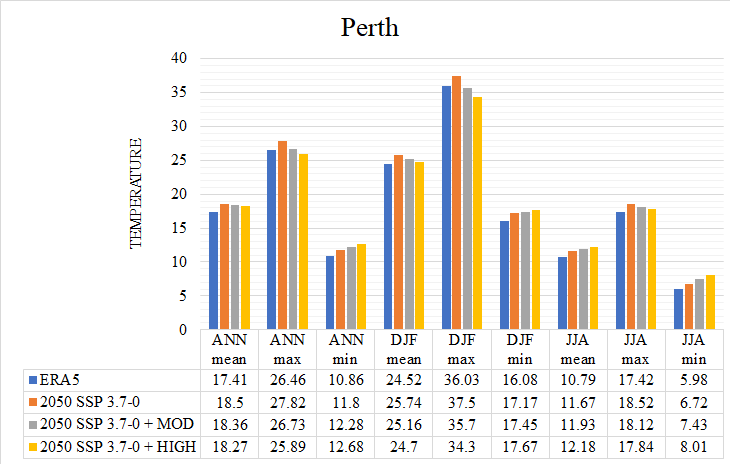
\includegraphics[trim={0 0 0 0},clip,scale=0.50]{images/image11.png}
\caption{\bf Mean daily, maximum (max) and minimum (min) temperatures for present day (ERA5), 2050 SSP3-7.5 emissions scenario, and the implementation of moderate (MON) and high (HIGH) IWM.}
 \label{fig:meandaily}
\end{figure}





\section{Conclusion}\label{sec:conclusion}


Using TARGET, an exploration of the impacts of IWM on urban climate, under both present-day climate and projected future conditions under climate change, has been completed. Some key findings are provided:

1. The use of TARGET, along with the use of LCZs for land surface cover data is an efficient and effective approach for modelling air temperatures in Australian cities. The approach captures both the inter-city and intra-city spatial variability of temperatures. The use of ERA5 data and the superimposed CMIP6 climate change data provides robust and consistent meteorological forcing data for TARGET.

2. Climate change will lead to warmer (mean daily, maximum, and minimum) temperatures across all Australian cities compared to BAU with the overall warming greatest for SSP5-8.5 for 2050. In Australian cities, summers are warming slightly more than annual temperatures, and winter temperatures slightly less.

3. The implementation of IWM modifies urban air temperatures. In general, IWM reduces mean daily maximum temperatures during the day, yet increases mean minimum temperatures at night. The net effect of this is a reduction in mean daily temperatures. The largest reductions in temperature from IWM are seen in the mean daily maximum temperatures during summer. 

4. Two scenarios of IWM implementation were explore based on current policy. The HIGH IWM scenario provided greater reductions in mean daily maximum air temperature. 

5. The impact of IWM on temperature varies between cities and is more evident in cities with a hotter and drier climate (such as Albury and Perth) resulting in large reduction in mean maximum temperature, particularly in summer. The impact of IWM on temperature is less evident in more humid, tropical cities (such as Darwin and Townsville). 

6. Impacts of IWM implementation on projected temperatures under climate change vary between cities, with larger reductions seen in cities with hotter and drier climates (as with BAU). The variations in temperature for each city resulting from IWM, are very similar under all climate change scenarios. 

7. IWM has the potential to offset warming from climate change. In hotter and drier cities, a MOD level of IWM implementation is effective in offsetting the projected mean maximum daily summer warming in 2050 under SSP3-7.0, and some of the warming in more humid, tropical cities. A HIGH level of IWM is needed to offset mean maximum daily summer warming in 2050 under SSP3-7 in humid, tropical cities.

8. IWM generally results in warmer night-time minimum temperatures. Other urban heat mitigation measures are needed to help offset this warming, particularly in summer. A range of options are available including increasing the albedo of urban surfaces (such as roofs and roads), controlling building heights and street widths, and reducing waste heat production (from building energy use and transport). These options could be explored in future work using TARGET and the approach used here.




%\subsection{Figures}
%Frontiers requires figures to be submitted individually, in the same order as they are referred to in the manuscript. Figures will then be automatically embedded at the bottom of the submitted manuscript. Kindly ensure that each table and figure is mentioned in the text and in numerical order. Figures must be of sufficient resolution for publication \href{http://home.frontiersin.org/about/author-guidelines#ResolutionRequirements}{see here for examples and minimum requirements}. Figures which are not according to the guidelines will cause substantial delay during the production process. Please see \href{http://home.frontiersin.org/about/author-guidelines#GeneralStyleGuidelinesforFigures}{here} for full figure guidelines. Cite figures with subfigures as figure \ref{fig:2}B.



%\subsection{Tables}
%Tables should be inserted at the end of the manuscript. Please build your table directly in LaTeX.Tables provided as jpeg/tiff files will not be accepted. Please note that very large tables (covering several pages) cannot be included in the final PDF for reasons of space. These tables will be published as \href{http://home.frontiersin.org/about/author-guidelines#SupplementaryMaterial}{Supplementary Material} on the online article page at the time of acceptance. The author will be notified during the typesetting of the final article if this is the case. 

%\section{Nomenclature}

%\subsection{Resource Identification Initiative}
%To take part in the Resource Identification Initiative, please use the corresponding catalog number and RRID in your current manuscript. For more information about the project and for steps on how to search for an RRID, please click \href{http://www.frontiersin.org/files/pdf/letter_to_author.pdf}{here}.

%\subsection{Life Science Identifiers}
%Life Science Identifiers (LSIDs) for ZOOBANK registered names or nomenclatural acts should be listed in the manuscript before the keywords. For more information on LSIDs please see \href{http://www.frontiersin.org/about/AuthorGuidelines#InclusionofZoologicalNomenclature}{Inclusion of Zoological Nomenclature} section of the guidelines.


%\section{Additional Requirements}
%
%For additional requirements for specific article types and further information please refer to \href{http://www.frontiersin.org/about/AuthorGuidelines#AdditionalRequirements}{Author Guidelines}.

\section*{Conflict of Interest Statement}
%All financial, commercial or other relationships that might be perceived by the academic community as representing a potential conflict of interest must be disclosed. If no such relationship exists, authors will be asked to confirm the following statement: 

The authors declare that the research was conducted in the absence of any commercial or financial relationships that could be construed as a potential conflict of interest.

\section*{Author Contributions}

The Author Contributions section is mandatory for all articles, including articles by sole authors. If an appropriate statement is not provided on submission, a standard one will be inserted during the production process. The Author Contributions statement must describe the contributions of individual authors referred to by their initials and, in doing so, all authors agree to be accountable for the content of the work. Please see  \href{http://home.frontiersin.org/about/author-guidelines#AuthorandContributors}{here} for full authorship criteria.

\section*{Funding}
Details of all funding sources should be provided, including grant numbers if applicable. Please ensure to add all necessary funding information, as after publication this is no longer possible.

\section*{Acknowledgments}
This is a short text to acknowledge the contributions of specific colleagues, institutions, or agencies that aided the efforts of the authors.

\section*{Supplemental Data}
 \href{http://home.frontiersin.org/about/author-guidelines#SupplementaryMaterial}{Supplementary Material} should be uploaded separately on submission, if there are Supplementary Figures, please include the caption in the same file as the figure. LaTeX Supplementary Material templates can be found in the Frontiers LaTeX folder.

\section*{Data Availability Statement}
The datasets [GENERATED/ANALYZED] for this study can be found in the [NAME OF REPOSITORY] [LINK].
% Please see the availability of data guidelines for more information, at https://www.frontiersin.org/about/author-guidelines#AvailabilityofData

\bibliographystyle{frontiersinSCNS_ENG_HUMS} % for Science, Engineering and Humanities and Social Sciences articles, for Humanities and Social Sciences articles please include page numbers in the in-text citations
%\bibliographystyle{frontiersinHLTH&FPHY} % for Health, Physics and Mathematics articles
\bibliography{Bib}

%%% Make sure to upload the bib file along with the tex file and PDF
%%% Please see the test.bib file for some examples of references

%\section*{Figure captions}
%
%%%% Please be aware that for original research articles we only permit a combined number of 15 figures and tables, one figure with multiple subfigures will count as only one figure.
%%%% Use this if adding the figures directly in the mansucript, if so, please remember to also upload the files when submitting your article
%%%% There is no need for adding the file termination, as long as you indicate where the file is saved. In the examples below the files (logo1.eps and logos.eps) are in the Frontiers LaTeX folder
%%%% If using *.tif files convert them to .jpg or .png
%%%%  NB logo1.eps is required in the path in order to correctly compile front page header %%%
%
%\begin{figure}[h!]
%\begin{center}
%
\includegraphics[width=10cm]{logo1}% This is a *.eps file
%\end{center}
%\caption{ Enter the caption for your figure here.  Repeat as  necessary for each of your figures}\label{fig:1}
%\end{figure}
%
%
%\begin{figure}[h!]
%\begin{center}
%\includegraphics[width=15cm]{logos}
%\end{center}
%\caption{This is a figure with sub figures, \textbf{(A)} is one logo, \textbf{(B)} is a different logo.}\label{fig:2}
%\end{figure}
%
%%%% If you are submitting a figure with subfigures please combine these into one image file with part labels integrated.
%%%% If you don't add the figures in the LaTeX files, please upload them when submitting the article.
%%%% Frontiers will add the figures at the end of the provisional pdf automatically
%%%% The use of LaTeX coding to draw Diagrams/Figures/Structures should be avoided. They should be external callouts including graphics.


\appendix
\setcounter{table}{0}
\renewcommand{\thetable}{A\arabic{table}}

\section{LCZ classes overview}\label{sec:appendix1}

\begin{figure}
\centering
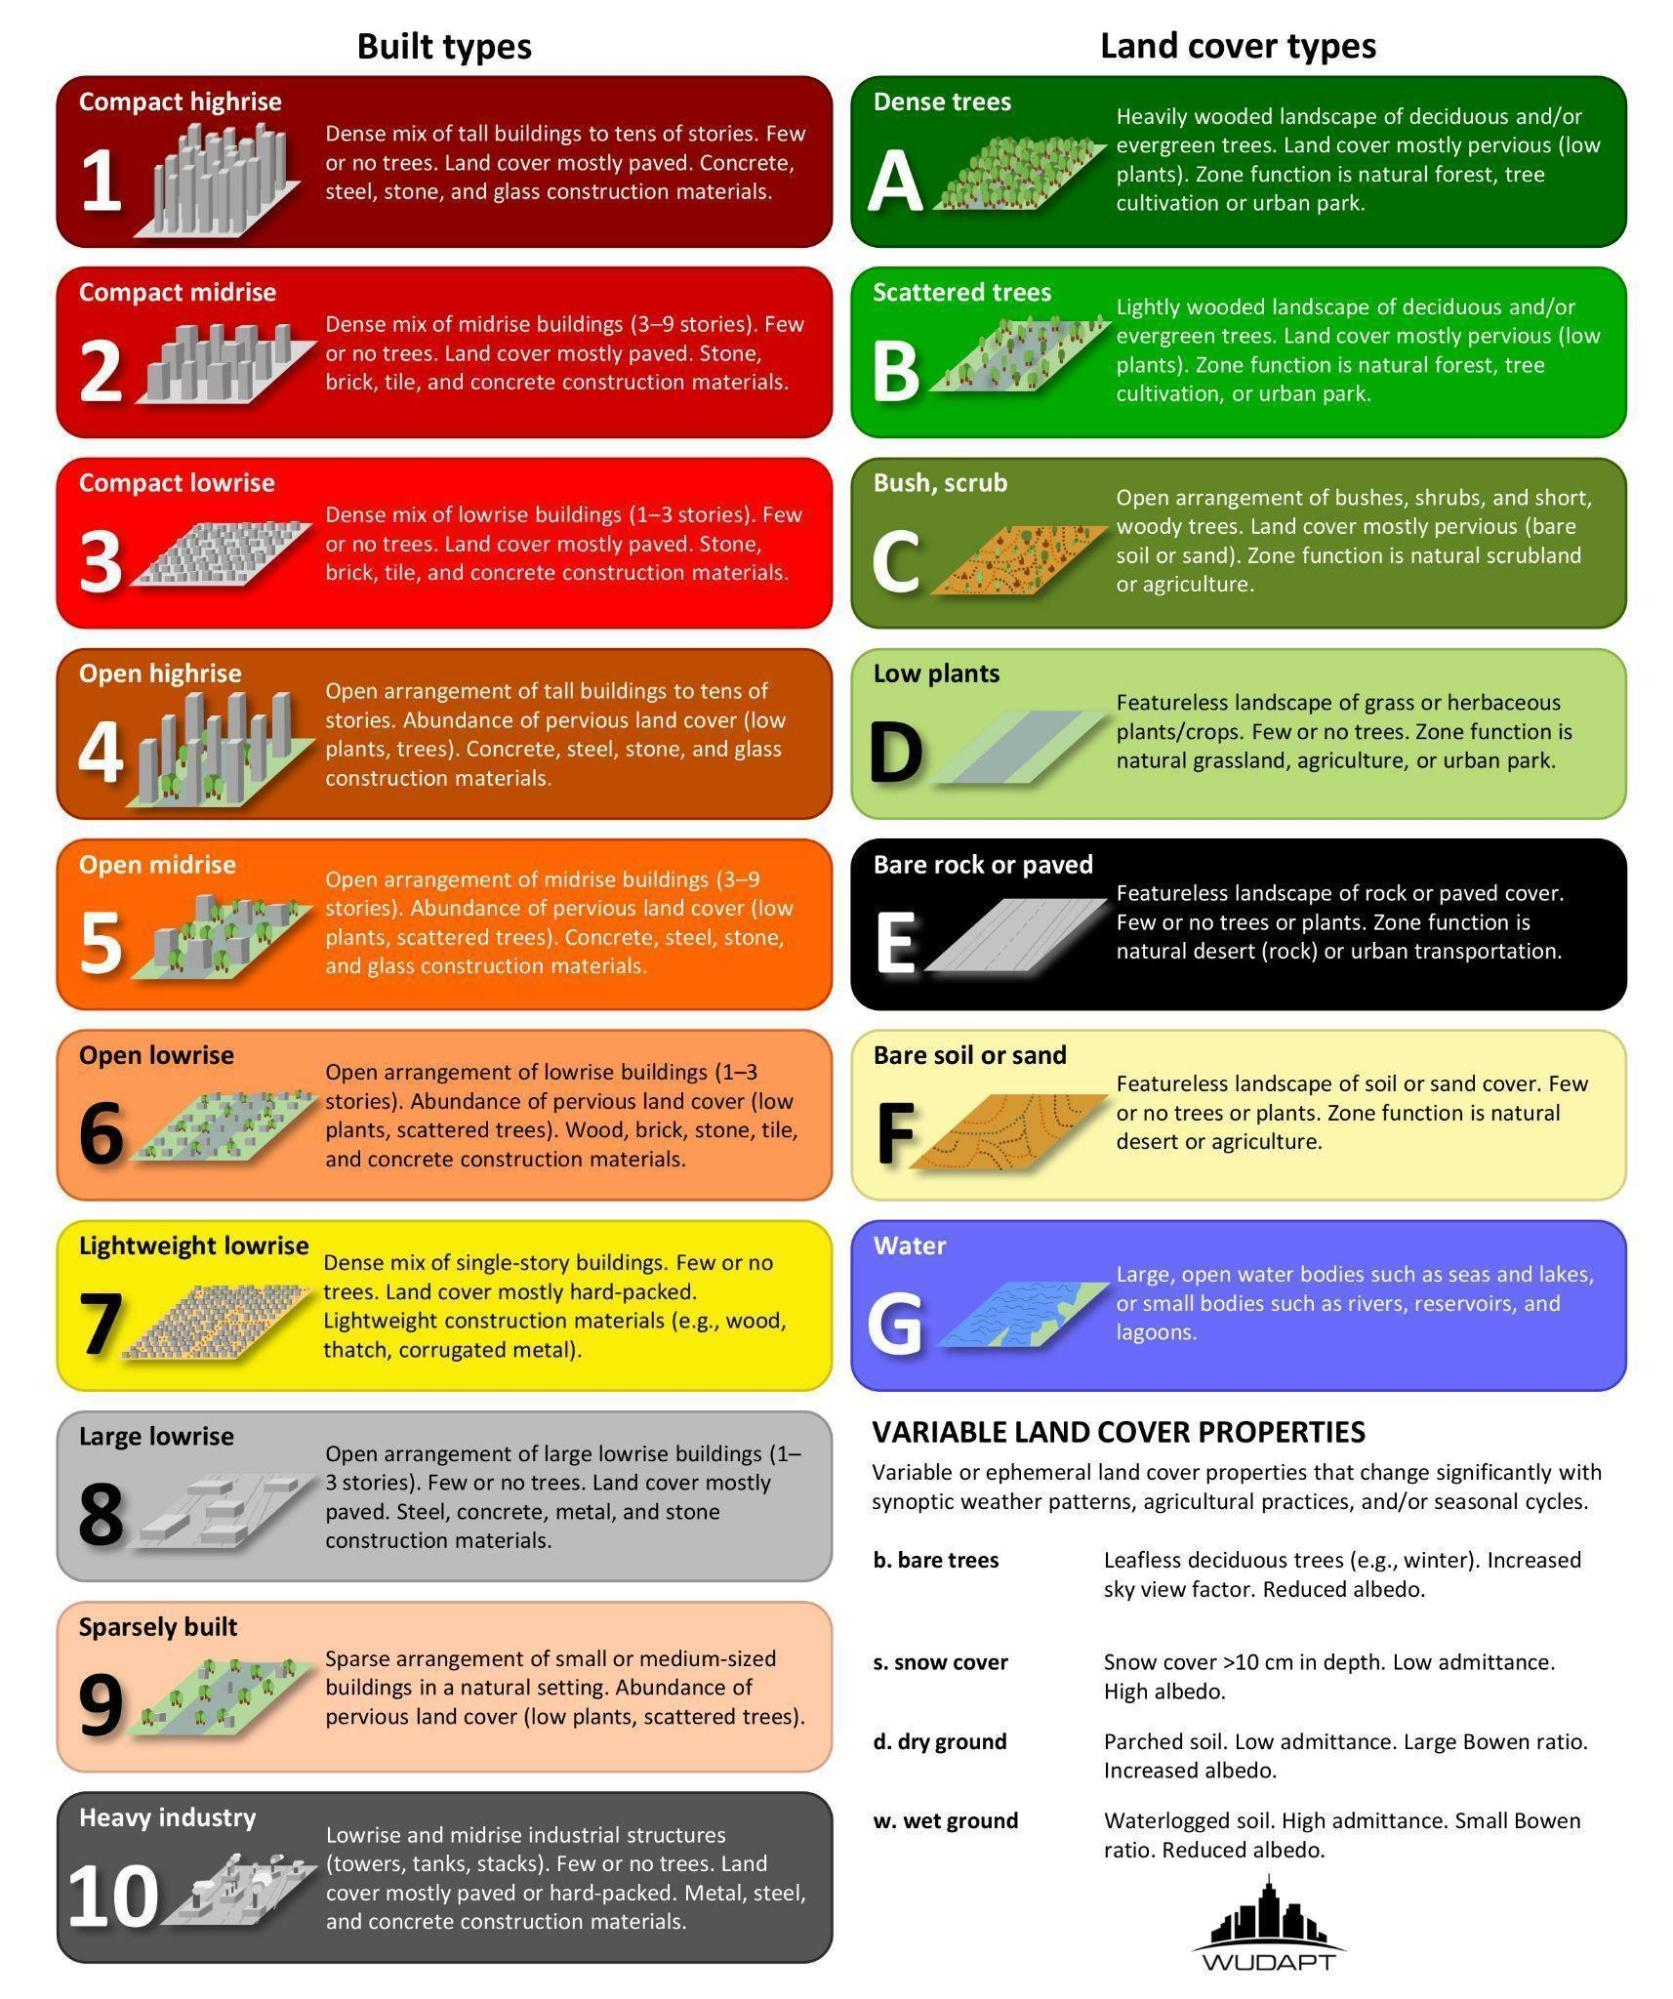
\includegraphics[trim={0 0 0 0},clip,scale=0.25]{images/image10.jpg}
\caption{\bf Overview of the 17 LCZ classes, adopted from \cite{Demuzere2022}}
 \label{fig:17lczs}
\end{figure}

\section{Results Table}\label{sec:appendix2}







%\setlength\arrayrulewidth{1pt} %Increasing linewidth 

\begin{landscape}
\begin{table}[!ht]\caption{Overview of results of TARGET modelling for Adelaide.}
\tiny   
    \begin{tabular}{|p{0.65cm}| p{0.4cm}| p{0.4cm}|p{0.4cm}|p{0.4cm}|p{0.4cm}|p{0.4cm}|p{0.4cm}|p{0.4cm}|p{0.4cm}|p{0.4cm}|p{0.4cm}|p{0.4cm}|p{0.4cm}|p{0.4cm}|p{0.4cm}|p{0.4cm}|p{0.4cm}|p{0.4cm}|p{0.4cm}|p{0.4cm}|p{0.4cm}|p{0.4cm}|p{0.4cm}|p{0.4cm}|p{0.4cm}|p{0.4cm}|p{0.4cm}|}
    \hline \multicolumn{28}{|c|}{ADELAIDE}\\
    \hline 
       ~ & \multicolumn{9}{c|}{Mean annual (ANN) daily temperature}
        & \multicolumn{9}{c|}{Mean summer (DJF) daily temperature} 
        &  \multicolumn{9}{c|}{Mean winter (JJA) daily temperature} 
         \\ \hline
        Scenario & BAU mean & BAU max & BAU   min & MOD mean & MOD max & MOD min & HIGH mean & HIGH max & HIGH   min & BAU mean & BAU     max & BAU     min & MOD mean & MOD max & MOD min & HIGH mean & HIGH max & HIGH   min & BAU    mean & BAU     max & BAU     min & MOD mean & MOD max & MOD min & HIGH mean & HIGH max & HIGH    min \\ \hline
        ERA5 & 15.81 & 24.03 & 9.56 & -0.19 & -0.97 & 0.3 & -0.31 & -1.67 & 0.55 & 23.12 & 33.67 & 14.77 & -0.62 & -1.67 & 0.12 & -1.1 & -2.91 & 0.22 & 8.86 & 14.83 & 4.57 & 0.2 & -0.33 & 0.51 & 0.41 & -0.54 & 0.92 \\ \hline
        2030 1-2.6 & 16.2 & 24.48 & 9.92 & -0.18 & -0.98 & 0.31 & -0.3 & -1.7 & 0.57 & 23.6 & 34.26 & 15.18 & -0.63 & -1.72 & 0.13 & -1.11 & -2.98 & 0.24 & 9.2 & 15.21 & 4.88 & 0.21 & -0.33 & 0.54 & 0.43 & -0.55 & 0.96 \\ \hline
        2030 3-7.0 & 16.27 & 24.55 & 9.98 & -0.18 & -0.98 & 0.31 & -0.3 & -1.7 & 0.57 & 23.64 & 34.31 & 15.21 & -0.63 & -1.72 & 0.13 & -1.11 & -2.98 & 0.24 & 9.28 & 15.3 & 4.95 & 0.22 & -0.33 & 0.54 & 0.43 & -0.54 & 0.97 \\ \hline
        2030 5-8.5 & 16.29 & 24.6 & 9.98 & -0.18 & -0.99 & 0.31 & -0.3 & -1.71 & 0.57 & 23.61 & 34.25 & 15.19 & -0.62 & -1.71 & 0.13 & -1.1 & -2.96 & 0.24 & 9.3 & 15.36 & 4.95 & 0.21 & -0.33 & 0.53 & 0.43 & -0.55 & 0.96 \\ \hline
        2050 1-2.6 & 16.45 & 24.82 & 10.12 & -0.19 & -1 & 0.32 & -0.3 & -1.72 & 0.58 & 23.84 & 34.52 & 15.41 & -0.63 & -1.73 & 0.13 & -1.11 & -2.98 & 0.24 & 9.41 & 15.52 & 5.03 & 0.21 & -0.33 & 0.54 & 0.43 & -0.55 & 0.96 \\ \hline
        2050 3-7.0 & 16.84 & 25.25 & 10.48 & -0.18 & -1.01 & 0.33 & -0.3 & -1.73 & 0.6 & 24.23 & 34.94 & 15.8 & -0.62 & -1.74 & 0.14 & -1.11 & -2.99 & 0.25 & 9.74 & 15.88 & 5.35 & 0.23 & -0.33 & 0.56 & 0.45 & -0.55 & 0.99 \\ \hline
        2050 5-8.5 & 16.92 & 25.33 & 10.57 & -0.18 & -1.01 & 0.33 & -0.29 & -1.73 & 0.61 & 24.29 & 35.01 & 15.85 & -0.62 & -1.74 & 0.15 & -1.1 & -2.99 & 0.26 & 9.83 & 15.97 & 5.43 & 0.23 & -0.33 & 0.56 & 0.46 & -0.55 & 1 \\ \hline
    \end{tabular}
\end{table}
%\setlength\arrayrulewidth{0.4pt} %Back to default



\begin{table}[!ht]\caption{Overview of results of TARGET modelling for Albury.}
  \tiny    
      \begin{tabular}{|p{0.65cm}| p{0.4cm}| p{0.4cm}|p{0.4cm}|p{0.4cm}|p{0.4cm}|p{0.4cm}|p{0.4cm}|p{0.4cm}|p{0.4cm}|p{0.4cm}|p{0.4cm}|p{0.4cm}|p{0.4cm}|p{0.4cm}|p{0.4cm}|p{0.4cm}|p{0.4cm}|p{0.4cm}|p{0.4cm}|p{0.4cm}|p{0.4cm}|p{0.4cm}|p{0.4cm}|p{0.4cm}|p{0.4cm}|p{0.4cm}|p{0.4cm}|}
      \hline \multicolumn{28}{|c|}{ALBURY}\\
      \hline 
         ~ & \multicolumn{9}{c|}{Mean annual (ANN) daily temperature}
          & \multicolumn{9}{c|}{Mean summer (DJF) daily temperature} 
          &  \multicolumn{9}{c|}{Mean winter (JJA) daily temperature} 
           \\ \hline
          Scenario & BAU mean & BAU max & BAU   min & MOD mean & MOD max & MOD min & HIGH mean & HIGH max & HIGH   min & BAU mean & BAU     max & BAU     min & MOD mean & MOD max & MOD min & HIGH mean & HIGH max & HIGH   min & BAU    mean & BAU     max & BAU     min & MOD mean & MOD max & MOD min & HIGH mean & HIGH max & HIGH    min \\ \hline
        ERA5 & 14.86 & 23.37 & 8.28 & -0.22 & -1.05 & 0.24 & -0.35 & -1.78 & 0.45 & 23.92 & 34.97 & 15.31 & -0.71 & -1.91 & 0.07 & -1.25 & -3.32 & 0.14 & 6.47 & 12.51 & 1.92 & 0.19 & -0.25 & 0.4 & 0.39 & -0.39 & 0.71 \\ \hline
        2030 1-2.6 & 15.34 & 23.95 & 8.71 & -0.21 & -1.06 & 0.26 & -0.35 & -1.81 & 0.48 & 24.47 & 35.66 & 15.78 & -0.71 & -1.93 & 0.08 & -1.26 & -3.38 & 0.16 & 6.88 & 13 & 2.27 & 0.2 & -0.25 & 0.41 & 0.41 & -0.39 & 0.74 \\ \hline
        2030 3-7.0 & 15.42 & 24 & 8.82 & -0.21 & -1.06 & 0.26 & -0.34 & -1.81 & 0.48 & 24.57 & 35.77 & 15.86 & -0.71 & -1.93 & 0.09 & -1.26 & -3.39 & 0.17 & 6.97 & 13.08 & 2.37 & 0.2 & -0.25 & 0.42 & 0.41 & -0.39 & 0.76 \\ \hline
        2030 5-8.5 & 15.44 & 24.04 & 8.81 & -0.21 & -1.06 & 0.26 & -0.35 & -1.81 & 0.48 & 24.57 & 35.73 & 15.88 & -0.71 & -1.92 & 0.08 & -1.26 & -3.37 & 0.17 & 6.98 & 13.11 & 2.39 & 0.2 & -0.25 & 0.41 & 0.41 & -0.39 & 0.75 \\ \hline
        2050 1-2.6 & 15.59 & 24.25 & 8.93 & -0.22 & -1.07 & 0.26 & -0.35 & -1.83 & 0.48 & 24.77 & 35.97 & 16.07 & -0.72 & -1.94 & 0.08 & -1.27 & -3.4 & 0.16 & 7.06 & 13.23 & 2.42 & 0.2 & -0.25 & 0.42 & 0.41 & -0.4 & 0.75 \\ \hline
        2050 3-7.0 & 16.13 & 24.83 & 9.47 & -0.21 & -1.08 & 0.28 & -0.34 & -1.84 & 0.52 & 25.38 & 36.64 & 16.64 & -0.72 & -1.95 & 0.11 & -1.28 & -3.43 & 0.21 & 7.54 & 13.78 & 2.87 & 0.21 & -0.26 & 0.44 & 0.44 & -0.4 & 0.8 \\ \hline
        2050 5-8.5 & 16.16 & 24.87 & 9.5 & -0.21 & -1.09 & 0.28 & -0.34 & -1.85 & 0.52 & 25.42 & 36.68 & 16.7 & -0.72 & -1.95 & 0.11 & -1.28 & -3.43 & 0.21 & 7.53 & 13.8 & 2.84 & 0.21 & -0.26 & 0.43 & 0.43 & -0.41 & 0.79 \\ \hline
    \end{tabular}
\end{table}




\begin{table}[!ht]\caption{Overview of results of TARGET modelling for Brisbane.}
\tiny    
    \begin{tabular}{|p{0.65cm}| p{0.4cm}| p{0.4cm}|p{0.4cm}|p{0.4cm}|p{0.4cm}|p{0.4cm}|p{0.4cm}|p{0.4cm}|p{0.4cm}|p{0.4cm}|p{0.4cm}|p{0.4cm}|p{0.4cm}|p{0.4cm}|p{0.4cm}|p{0.4cm}|p{0.4cm}|p{0.4cm}|p{0.4cm}|p{0.4cm}|p{0.4cm}|p{0.4cm}|p{0.4cm}|p{0.4cm}|p{0.4cm}|p{0.4cm}|p{0.4cm}|}
    \hline \multicolumn{28}{|c|}{BRISBANE}\\
    \hline 
       ~ & \multicolumn{9}{c|}{Mean annual (ANN) daily temperature}
        & \multicolumn{9}{c|}{Mean summer (DJF) daily temperature} 
        &  \multicolumn{9}{c|}{Mean winter (JJA) daily temperature} 
         \\ \hline
        Scenario & BAU mean & BAU max & BAU   min & MOD mean & MOD max & MOD min & HIGH mean & HIGH max & HIGH   min & BAU mean & BAU     max & BAU     min & MOD mean & MOD max & MOD min & HIGH mean & HIGH max & HIGH   min & BAU    mean & BAU     max & BAU     min & MOD mean & MOD max & MOD min & HIGH mean & HIGH max & HIGH    min \\ \hline
        ERA5 & 19.86 & 26.91 & 14.49 & -0.09 & -0.56 & 0.15 & -0.12 & -0.86 & 0.28 & 24.99 & 32.03 & 19.77 & -0.27 & -0.77 & 0.08 & -0.43 & -1.21 & 0.16 & 14.03 & 21.18 & 8.41 & 0.07 & -0.36 & 0.26 & 0.17 & -0.59 & 0.46 \\ \hline
        2030 1-2.6 & 20.31 & 27.43 & 14.9 & -0.08 & -0.56 & 0.17 & -0.11 & -0.87 & 0.3 & 25.49 & 32.61 & 20.2 & -0.26 & -0.76 & 0.1 & -0.42 & -1.21 & 0.19 & 14.45 & 21.64 & 8.83 & 0.08 & -0.36 & 0.28 & 0.18 & -0.59 & 0.49 \\ \hline
        2030 3-7.0 & 20.44 & 27.56 & 15.04 & -0.08 & -0.56 & 0.17 & -0.11 & -0.87 & 0.31 & 25.56 & 32.68 & 20.29 & -0.26 & -0.76 & 0.11 & -0.41 & -1.21 & 0.2 & 14.65 & 21.85 & 9.02 & 0.09 & -0.36 & 0.29 & 0.19 & -0.6 & 0.5 \\ \hline
        2030 5-8.5 & 20.44 & 27.55 & 15.05 & -0.08 & -0.56 & 0.17 & -0.11 & -0.87 & 0.31 & 25.55 & 32.66 & 20.27 & -0.26 & -0.76 & 0.11 & -0.41 & -1.21 & 0.2 & 14.66 & 21.89 & 9.01 & 0.09 & -0.37 & 0.28 & 0.19 & -0.6 & 0.5 \\ \hline
        2050 1-2.6 & 20.57 & 27.73 & 15.15 & -0.08 & -0.56 & 0.18 & -0.11 & -0.88 & 0.32 & 25.72 & 32.91 & 20.4 & -0.26 & -0.77 & 0.11 & -0.42 & -1.23 & 0.2 & 14.74 & 21.93 & 9.12 & 0.09 & -0.36 & 0.29 & 0.19 & -0.59 & 0.51 \\ \hline
        2050 3-7.0 & 20.99 & 28.13 & 15.59 & -0.07 & -0.57 & 0.2 & -0.09 & -0.88 & 0.35 & 26 & 33.11 & 20.72 & -0.24 & -0.77 & 0.13 & -0.39 & -1.21 & 0.24 & 15.27 & 22.48 & 9.65 & 0.1 & -0.36 & 0.32 & 0.22 & -0.6 & 0.56 \\ \hline
        2050 5-8.5 & 21.08 & 28.24 & 15.67 & -0.07 & -0.57 & 0.2 & -0.09 & -0.89 & 0.35 & 26.16 & 33.26 & 20.87 & -0.24 & -0.76 & 0.14 & -0.39 & -1.23 & 0.25 & 15.27 & 22.52 & 9.65 & 0.1 & -0.37 & 0.3 & 0.21 & -0.6 & 0.53 \\ \hline
    \end{tabular}
\end{table}
\end{landscape}


\begin{landscape}
\begin{table}[!ht]\caption{Overview of results of TARGET modelling for Canberra.}
\tiny    
    \begin{tabular}{|p{0.65cm}| p{0.4cm}| p{0.4cm}|p{0.4cm}|p{0.4cm}|p{0.4cm}|p{0.4cm}|p{0.4cm}|p{0.4cm}|p{0.4cm}|p{0.4cm}|p{0.4cm}|p{0.4cm}|p{0.4cm}|p{0.4cm}|p{0.4cm}|p{0.4cm}|p{0.4cm}|p{0.4cm}|p{0.4cm}|p{0.4cm}|p{0.4cm}|p{0.4cm}|p{0.4cm}|p{0.4cm}|p{0.4cm}|p{0.4cm}|p{0.4cm}|}
    \hline \multicolumn{28}{|c|}{CANBERRA}\\
    \hline 
       ~ & \multicolumn{9}{c|}{Mean annual (ANN) daily temperature}
        & \multicolumn{9}{c|}{Mean summer (DJF) daily temperature} 
        &  \multicolumn{9}{c|}{Mean winter (JJA) daily temperature} 
         \\ \hline
        Scenario & BAU mean & BAU max & BAU   min & MOD mean & MOD max & MOD min & HIGH mean & HIGH max & HIGH   min & BAU mean & BAU     max & BAU     min & MOD mean & MOD max & MOD min & HIGH mean & HIGH max & HIGH   min & BAU    mean & BAU     max & BAU     min & MOD mean & MOD max & MOD min & HIGH mean & HIGH max & HIGH    min \\ \hline
        ERA5 & 12.64 & 21.23 & 6.22 & -0.18 & -0.96 & 0.23 & -0.29 & -1.63 & 0.42 & 20.72 & 31.22 & 12.79 & -0.6 & -1.68 & 0.09 & -1.05 & -2.88 & 0.18 & 4.81 & 11.38 & -0.02 & 0.19 & -0.28 & 0.39 & 0.38 & -0.44 & 0.66 \\ \hline
        2030 1-2.6 & 13.14 & 21.83 & 6.67 & -0.18 & -0.98 & 0.25 & -0.29 & -1.67 & 0.45 & 21.34 & 31.99 & 13.33 & -0.61 & -1.72 & 0.1 & -1.06 & -2.96 & 0.21 & 5.22 & 11.86 & 0.37 & 0.19 & -0.28 & 0.4 & 0.39 & -0.44 & 0.69 \\ \hline
        2030 3-7.0 & 13.22 & 21.9 & 6.75 & -0.18 & -0.97 & 0.25 & -0.28 & -1.66 & 0.45 & 21.39 & 32.04 & 13.38 & -0.6 & -1.71 & 0.11 & -1.06 & -2.95 & 0.22 & 5.35 & 12.06 & 0.45 & 0.19 & -0.29 & 0.39 & 0.39 & -0.45 & 0.68 \\ \hline
        2030 5-8.5 & 13.25 & 21.93 & 6.79 & -0.18 & -0.98 & 0.25 & -0.29 & -1.66 & 0.45 & 21.4 & 32.05 & 13.4 & -0.6 & -1.71 & 0.11 & -1.06 & -2.95 & 0.21 & 5.34 & 12 & 0.48 & 0.19 & -0.28 & 0.39 & 0.39 & -0.45 & 0.68 \\ \hline
        2050 1-2.6 & 13.39 & 22.16 & 6.87 & -0.18 & -1 & 0.25 & -0.29 & -1.69 & 0.45 & 21.59 & 32.29 & 13.56 & -0.61 & -1.74 & 0.11 & -1.07 & -2.99 & 0.22 & 5.43 & 12.18 & 0.52 & 0.19 & -0.29 & 0.38 & 0.39 & -0.45 & 0.67 \\ \hline
        2050 3-7.0 & 13.86 & 22.6 & 7.38 & -0.17 & -0.97 & 0.27 & -0.27 & -1.67 & 0.49 & 22 & 32.69 & 13.99 & -0.6 & -1.71 & 0.12 & -1.05 & -2.96 & 0.24 & 5.91 & 12.71 & 0.98 & 0.2 & -0.28 & 0.41 & 0.4 & -0.45 & 0.71 \\ \hline
        2050 5-8.5 & 13.93 & 22.73 & 7.41 & -0.17 & -0.99 & 0.27 & -0.28 & -1.69 & 0.48 & 22.07 & 32.72 & 14.06 & -0.6 & -1.7 & 0.12 & -1.05 & -2.95 & 0.24 & 5.92 & 12.8 & 0.95 & 0.2 & -0.29 & 0.41 & 0.4 & -0.46 & 0.7 \\ \hline
    \end{tabular}
\end{table}




\begin{table}[!ht]\caption{Overview of results of TARGET modelling for Darwin.}
\tiny    
    \begin{tabular}{|p{0.65cm}| p{0.4cm}| p{0.4cm}|p{0.4cm}|p{0.4cm}|p{0.4cm}|p{0.4cm}|p{0.4cm}|p{0.4cm}|p{0.4cm}|p{0.4cm}|p{0.4cm}|p{0.4cm}|p{0.4cm}|p{0.4cm}|p{0.4cm}|p{0.4cm}|p{0.4cm}|p{0.4cm}|p{0.4cm}|p{0.4cm}|p{0.4cm}|p{0.4cm}|p{0.4cm}|p{0.4cm}|p{0.4cm}|p{0.4cm}|p{0.4cm}|}
    \hline \multicolumn{28}{|c|}{DARWIN}\\
    \hline 
       ~ & \multicolumn{9}{c|}{Mean annual (ANN) daily temperature}
        & \multicolumn{9}{c|}{Mean summer (DJF) daily temperature} 
        &  \multicolumn{9}{c|}{Mean winter (JJA) daily temperature} 
         \\ \hline
        Scenario & BAU mean & BAU max & BAU   min & MOD mean & MOD max & MOD min & HIGH mean & HIGH max & HIGH   min & BAU mean & BAU     max & BAU     min & MOD mean & MOD max & MOD min & HIGH mean & HIGH max & HIGH   min & BAU    mean & BAU     max & BAU     min & MOD mean & MOD max & MOD min & HIGH mean & HIGH max & HIGH    min \\ \hline
        ERA5 & 27.33 & 33.99 & 22.39 & -0.12 & -0.51 & 0.08 & -0.18 & -0.77 & 0.14 & 28.24 & 33.56 & 24.64 & -0.13 & -0.49 & 0.1 & -0.19 & -0.77 & 0.19 & 24.63 & 32.6 & 18.36 & -0.07 & -0.45 & 0.1 & -0.1 & -0.67 & 0.17 \\ \hline
        2030 1-2.6 & 27.84 & 34.55 & 22.89 & -0.12 & -0.51 & 0.09 & -0.17 & -0.77 & 0.16 & 28.68 & 34.04 & 25.04 & -0.12 & -0.48 & 0.11 & -0.17 & -0.76 & 0.22 & 25.21 & 33.25 & 18.93 & -0.07 & -0.45 & 0.11 & -0.1 & -0.67 & 0.18 \\ \hline
        2030 3-7.0 & 27.95 & 34.62 & 23.03 & -0.11 & -0.51 & 0.09 & -0.17 & -0.77 & 0.16 & 28.77 & 34.14 & 25.14 & -0.12 & -0.49 & 0.12 & -0.17 & -0.77 & 0.23 & 25.3 & 33.28 & 19.07 & -0.06 & -0.45 & 0.11 & -0.09 & -0.67 & 0.18 \\ \hline
        2030 5-8.5 & 27.94 & 34.62 & 23.01 & -0.12 & -0.51 & 0.09 & -0.17 & -0.77 & 0.16 & 28.8 & 34.17 & 25.16 & -0.12 & -0.48 & 0.12 & -0.17 & -0.77 & 0.23 & 25.33 & 33.34 & 19.09 & -0.06 & -0.45 & 0.11 & -0.09 & -0.67 & 0.18 \\ \hline
        2050 1-2.6 & 28.08 & 34.81 & 23.12 & -0.11 & -0.51 & 0.09 & -0.17 & -0.77 & 0.16 & 28.91 & 34.29 & 25.25 & -0.12 & -0.49 & 0.12 & -0.17 & -0.77 & 0.24 & 25.45 & 33.48 & 19.19 & -0.06 & -0.45 & 0.11 & -0.09 & -0.67 & 0.18 \\ \hline
        2050 3-7.0 & 28.53 & 35.21 & 23.62 & -0.11 & -0.51 & 0.11 & -0.16 & -0.77 & 0.19 & 29.31 & 34.72 & 25.64 & -0.11 & -0.48 & 0.14 & -0.15 & -0.77 & 0.26 & 26.02 & 34 & 19.85 & -0.06 & -0.45 & 0.13 & -0.08 & -0.68 & 0.2 \\ \hline
        2050 5-8.5 & 28.62 & 35.31 & 23.69 & -0.11 & -0.5 & 0.11 & -0.16 & -0.77 & 0.19 & 29.39 & 34.84 & 25.69 & -0.11 & -0.48 & 0.14 & -0.15 & -0.77 & 0.27 & 26.13 & 34.12 & 19.95 & -0.06 & -0.45 & 0.13 & -0.08 & -0.68 & 0.2 \\ \hline
    \end{tabular}
\end{table}



\begin{table}[!ht]\caption{Overview of results of TARGET modelling for Melbourne.}
\tiny    
    \begin{tabular}{|p{0.65cm}| p{0.4cm}| p{0.4cm}|p{0.4cm}|p{0.4cm}|p{0.4cm}|p{0.4cm}|p{0.4cm}|p{0.4cm}|p{0.4cm}|p{0.4cm}|p{0.4cm}|p{0.4cm}|p{0.4cm}|p{0.4cm}|p{0.4cm}|p{0.4cm}|p{0.4cm}|p{0.4cm}|p{0.4cm}|p{0.4cm}|p{0.4cm}|p{0.4cm}|p{0.4cm}|p{0.4cm}|p{0.4cm}|p{0.4cm}|p{0.4cm}|}
    \hline \multicolumn{28}{|c|}{MELBOURNE}\\
    \hline 
       ~ & \multicolumn{9}{c|}{Mean annual (ANN) daily temperature}
        & \multicolumn{9}{c|}{Mean summer (DJF) daily temperature} 
        &  \multicolumn{9}{c|}{Mean winter (JJA) daily temperature} 
         \\ \hline
        Scenario & BAU mean & BAU max & BAU   min & MOD mean & MOD max & MOD min & HIGH mean & HIGH max & HIGH   min & BAU mean & BAU     max & BAU     min & MOD mean & MOD max & MOD min & HIGH mean & HIGH max & HIGH   min & BAU    mean & BAU     max & BAU     min & MOD mean & MOD max & MOD min & HIGH mean & HIGH max & HIGH    min \\ \hline
        ERA5 & 14.34 & 20.79 & 9.29 & -0.14 & -0.82 & 0.28 & -0.21 & -1.43 & 0.51 & 20.43 & 28.42 & 13.91 & -0.57 & -1.42 & 0.05 & -1 & -2.53 & 0.11 & 8.37 & 13.32 & 4.8 & 0.27 & -0.25 & 0.55 & 0.53 & -0.41 & 0.99 \\ \hline
        2030 1-2.6 & 14.64 & 22.03 & 9.08 & -0.11 & -0.85 & 0.37 & -0.15 & -1.43 & 0.67 & 21.01 & 30.25 & 13.8 & -0.55 & -1.45 & 0.11 & -0.94 & -2.48 & 0.22 & 8.4 & 14 & 4.42 & 0.3 & -0.28 & 0.66 & 0.6 & -0.44 & 1.21 \\ \hline
        2030 3-7.0 & 14.74 & 22.13 & 9.19 & -0.11 & -0.85 & 0.37 & -0.15 & -1.43 & 0.68 & 21.13 & 30.36 & 13.94 & -0.54 & -1.44 & 0.12 & -0.93 & -2.47 & 0.22 & 8.5 & 14.1 & 4.51 & 0.3 & -0.28 & 0.67 & 0.61 & -0.44 & 1.22 \\ \hline
        2030 5-8.5 & 14.78 & 22.22 & 9.18 & -0.11 & -0.86 & 0.37 & -0.15 & -1.45 & 0.67 & 21.19 & 30.52 & 13.92 & -0.55 & -1.47 & 0.11 & -0.95 & -2.52 & 0.22 & 8.5 & 14.13 & 4.49 & 0.3 & -0.28 & 0.67 & 0.61 & -0.44 & 1.21 \\ \hline
        2050 1-2.6 & 14.92 & 22.37 & 9.32 & -0.11 & -0.86 & 0.37 & -0.15 & -1.45 & 0.68 & 21.35 & 30.68 & 14.1 & -0.55 & -1.45 & 0.12 & -0.94 & -2.51 & 0.23 & 8.59 & 14.21 & 4.58 & 0.31 & -0.28 & 0.68 & 0.62 & -0.43 & 1.22 \\ \hline
        2050 3-7.0 & 15.4 & 22.91 & 9.77 & -0.1 & -0.87 & 0.4 & -0.13 & -1.47 & 0.72 & 21.94 & 31.39 & 14.62 & -0.55 & -1.49 & 0.13 & -0.95 & -2.58 & 0.25 & 9.03 & 14.7 & 5 & 0.33 & -0.28 & 0.7 & 0.65 & -0.43 & 1.28 \\ \hline
        2050 5-8.5 & 15.39 & 22.88 & 9.79 & -0.1 & -0.86 & 0.4 & -0.13 & -1.46 & 0.72 & 21.91 & 31.29 & 14.64 & -0.55 & -1.47 & 0.14 & -0.94 & -2.56 & 0.25 & 8.99 & 14.66 & 4.97 & 0.33 & -0.28 & 0.71 & 0.65 & -0.43 & 1.28 \\ \hline
    \end{tabular}
\end{table}
\end{landscape}



\begin{landscape}
\begin{table}[!ht]\caption{Overview of results of TARGET modelling for Perth.}
\tiny    
    \begin{tabular}{|p{0.65cm}| p{0.4cm}| p{0.4cm}|p{0.4cm}|p{0.4cm}|p{0.4cm}|p{0.4cm}|p{0.4cm}|p{0.4cm}|p{0.4cm}|p{0.4cm}|p{0.4cm}|p{0.4cm}|p{0.4cm}|p{0.4cm}|p{0.4cm}|p{0.4cm}|p{0.4cm}|p{0.4cm}|p{0.4cm}|p{0.4cm}|p{0.4cm}|p{0.4cm}|p{0.4cm}|p{0.4cm}|p{0.4cm}|p{0.4cm}|p{0.4cm}|}
    \hline \multicolumn{28}{|c|}{PERTH}\\
    \hline 
       ~ & \multicolumn{9}{c|}{Mean annual (ANN) daily temperature}
        & \multicolumn{9}{c|}{Mean summer (DJF) daily temperature} 
        &  \multicolumn{9}{c|}{Mean winter (JJA) daily temperature} 
         \\ \hline
        Scenario & BAU mean & BAU max & BAU   min & MOD mean & MOD max & MOD min & HIGH mean & HIGH max & HIGH   min & BAU mean & BAU     max & BAU     min & MOD mean & MOD max & MOD min & HIGH mean & HIGH max & HIGH   min & BAU    mean & BAU     max & BAU     min & MOD mean & MOD max & MOD min & HIGH mean & HIGH max & HIGH    min \\ \hline
        ERA5 & 17.41 & 26.46 & 10.86 & -0.15 & -1.05 & 0.43 & -0.25 & -1.86 & 0.8 & 24.52 & 36.03 & 16.08 & -0.58 & -1.74 & 0.23 & -1.04 & -3.12 & 0.42 & 10.79 & 17.42 & 5.98 & 0.24 & -0.39 & 0.66 & 0.47 & -0.67 & 1.21 \\ \hline
        2030 1-2.6 & 17.85 & 27.01 & 11.24 & -0.15 & -1.06 & 0.45 & -0.24 & -1.89 & 0.83 & 25 & 36.59 & 16.53 & -0.58 & -1.76 & 0.25 & -1.04 & -3.15 & 0.45 & 11.14 & 17.85 & 6.27 & 0.25 & -0.39 & 0.68 & 0.49 & -0.67 & 1.25 \\ \hline
        2030 3-7.0 & 17.92 & 27.1 & 11.31 & -0.14 & -1.07 & 0.46 & -0.24 & -1.89 & 0.83 & 25.11 & 36.76 & 16.61 & -0.58 & -1.78 & 0.25 & -1.04 & -3.17 & 0.46 & 11.24 & 18 & 6.34 & 0.25 & -0.4 & 0.69 & 0.49 & -0.68 & 1.25 \\ \hline
        2030 5-8.5 & 17.96 & 27.15 & 11.35 & -0.14 & -1.07 & 0.46 & -0.24 & -1.89 & 0.84 & 25.08 & 36.68 & 16.6 & -0.57 & -1.76 & 0.25 & -1.03 & -3.15 & 0.46 & 11.27 & 18.03 & 6.37 & 0.25 & -0.4 & 0.69 & 0.49 & -0.68 & 1.26 \\ \hline
        2050 1-2.6 & 18.07 & 27.3 & 11.43 & -0.14 & -1.08 & 0.46 & -0.24 & -1.91 & 0.84 & 25.23 & 36.87 & 16.73 & -0.57 & -1.78 & 0.26 & -1.04 & -3.17 & 0.47 & 11.33 & 18.08 & 6.44 & 0.25 & -0.4 & 0.69 & 0.5 & -0.67 & 1.26 \\ \hline
        2050 3-7.0 & 18.5 & 27.82 & 11.8 & -0.14 & -1.09 & 0.48 & -0.23 & -1.93 & 0.88 & 25.74 & 37.5 & 17.17 & -0.58 & -1.8 & 0.28 & -1.04 & -3.2 & 0.5 & 11.67 & 18.52 & 6.72 & 0.26 & -0.4 & 0.71 & 0.51 & -0.68 & 1.29 \\ \hline
        2050 5-8.5 & 18.61 & 27.94 & 11.92 & -0.13 & -1.1 & 0.49 & -0.22 & -1.93 & 0.89 & 25.9 & 37.67 & 17.34 & -0.57 & -1.8 & 0.28 & -1.03 & -3.21 & 0.52 & 11.75 & 18.59 & 6.8 & 0.27 & -0.39 & 0.72 & 0.52 & -0.67 & 1.3 \\ \hline
    \end{tabular}
\end{table}




\begin{table}[!ht]\caption{Overview of results of TARGET modelling for Sydney.}
\tiny    
    \begin{tabular}{|p{0.65cm}| p{0.4cm}| p{0.4cm}|p{0.4cm}|p{0.4cm}|p{0.4cm}|p{0.4cm}|p{0.4cm}|p{0.4cm}|p{0.4cm}|p{0.4cm}|p{0.4cm}|p{0.4cm}|p{0.4cm}|p{0.4cm}|p{0.4cm}|p{0.4cm}|p{0.4cm}|p{0.4cm}|p{0.4cm}|p{0.4cm}|p{0.4cm}|p{0.4cm}|p{0.4cm}|p{0.4cm}|p{0.4cm}|p{0.4cm}|p{0.4cm}|}
    \hline \multicolumn{28}{|c|}{SYDNEY}\\
    \hline 
       ~ & \multicolumn{9}{c|}{Mean annual (ANN) daily temperature}
        & \multicolumn{9}{c|}{Mean summer (DJF) daily temperature} 
        &  \multicolumn{9}{c|}{Mean winter (JJA) daily temperature} 
         \\ \hline
        Scenario & BAU mean & BAU max & BAU   min & MOD mean & MOD max & MOD min & HIGH mean & HIGH max & HIGH   min & BAU mean & BAU     max & BAU     min & MOD mean & MOD max & MOD min & HIGH mean & HIGH max & HIGH   min & BAU    mean & BAU     max & BAU     min & MOD mean & MOD max & MOD min & HIGH mean & HIGH max & HIGH    min \\ \hline
        ERA5 & 17.01 & 25.49 & 10.83 & -0.14 & -0.89 & 0.24 & -0.22 & -1.49 & 0.45 & 23.49 & 32.78 & 16.83 & -0.43 & -1.35 & 0.13 & -0.74 & -2.32 & 0.27 & 10.22 & 17.87 & 4.62 & 0.13 & -0.41 & 0.34 & 0.26 & -0.68 & 0.62 \\ \hline
        2030 1-2.6 & 17.5 & 26.06 & 11.26 & -0.14 & -0.9 & 0.25 & -0.21 & -1.51 & 0.47 & 24.05 & 33.45 & 17.31 & -0.43 & -1.38 & 0.15 & -0.75 & -2.37 & 0.29 & 10.63 & 18.33 & 4.99 & 0.13 & -0.41 & 0.35 & 0.28 & -0.67 & 0.64 \\ \hline
        2030 3-7.0 & 17.58 & 26.12 & 11.35 & -0.13 & -0.89 & 0.26 & -0.21 & -1.5 & 0.48 & 24.09 & 33.45 & 17.37 & -0.43 & -1.35 & 0.15 & -0.73 & -2.33 & 0.3 & 10.79 & 18.57 & 5.13 & 0.13 & -0.42 & 0.36 & 0.28 & -0.7 & 0.65 \\ \hline
        2030 5-8.5 & 17.61 & 26.15 & 11.39 & -0.13 & -0.89 & 0.26 & -0.21 & -1.51 & 0.48 & 24.1 & 33.46 & 17.37 & -0.43 & -1.35 & 0.15 & -0.73 & -2.33 & 0.31 & 10.75 & 18.47 & 5.11 & 0.14 & -0.41 & 0.36 & 0.28 & -0.68 & 0.65 \\ \hline
        2050 1-2.6 & 17.75 & 26.37 & 11.48 & -0.14 & -0.91 & 0.26 & -0.21 & -1.53 & 0.48 & 24.29 & 33.75 & 17.51 & -0.43 & -1.39 & 0.15 & -0.74 & -2.38 & 0.31 & 10.86 & 18.64 & 5.18 & 0.14 & -0.42 & 0.36 & 0.29 & -0.69 & 0.65 \\ \hline
        2050 3-7.0 & 18.2 & 26.81 & 11.94 & -0.12 & -0.9 & 0.28 & -0.19 & -1.52 & 0.52 & 24.69 & 34.09 & 17.93 & -0.42 & -1.35 & 0.17 & -0.73 & -2.34 & 0.34 & 11.37 & 19.19 & 5.67 & 0.15 & -0.42 & 0.38 & 0.31 & -0.69 & 0.69 \\ \hline
        2050 5-8.5 & 18.29 & 26.94 & 12 & -0.13 & -0.9 & 0.28 & -0.19 & -1.53 & 0.52 & 24.77 & 34.16 & 18.02 & -0.42 & -1.35 & 0.17 & -0.72 & -2.32 & 0.34 & 11.36 & 19.22 & 5.63 & 0.15 & -0.41 & 0.37 & 0.3 & -0.7 & 0.68 \\ \hline
    \end{tabular}
\end{table}



\begin{table}[!ht]\caption{Overview of results of TARGET modelling for Townsville.}
\tiny
    \begin{tabular}{|p{0.65cm}| p{0.4cm}| p{0.4cm}|p{0.4cm}|p{0.4cm}|p{0.4cm}|p{0.4cm}|p{0.4cm}|p{0.4cm}|p{0.4cm}|p{0.4cm}|p{0.4cm}|p{0.4cm}|p{0.4cm}|p{0.4cm}|p{0.4cm}|p{0.4cm}|p{0.4cm}|p{0.4cm}|p{0.4cm}|p{0.4cm}|p{0.4cm}|p{0.4cm}|p{0.4cm}|p{0.4cm}|p{0.4cm}|p{0.4cm}|p{0.4cm}|}
    \hline \multicolumn{28}{|c|}{Townsville}\\
    \hline 
       ~ & \multicolumn{9}{c|}{Mean annual (ANN) daily temperature}
        & \multicolumn{9}{c|}{Mean summer (DJF) daily temperature} 
        &  \multicolumn{9}{c|}{Mean winter (JJA) daily temperature} 
         \\ \hline
        Scenario & BAU mean & BAU max & BAU   min & MOD mean & MOD max & MOD min & HIGH mean & HIGH max & HIGH   min & BAU mean & BAU     max & BAU     min & MOD mean & MOD max & MOD min & HIGH mean & HIGH max & HIGH   min & BAU    mean & BAU     max & BAU     min & MOD mean & MOD max & MOD min & HIGH mean & HIGH max & HIGH    min \\ \hline
        ERA5 & 23.54 & 29.46 & 18.89 & -0.11 & -0.41 & 0.07 & -0.17 & -0.62 & 0.12 & 27.45 & 33.28 & 23.03 & -0.22 & -0.59 & 0.07 & -0.35 & -0.93 & 0.14 & 18.82 & 25.04 & 13.69 & 0 & -0.26 & 0.11 & 0.03 & -0.38 & 0.2 \\ \hline
        2030 1-2.6 & 24.01 & 29.98 & 19.31 & -0.11 & -0.41 & 0.08 & -0.16 & -0.63 & 0.14 & 27.87 & 33.76 & 23.41 & -0.21 & -0.59 & 0.09 & -0.34 & -0.93 & 0.17 & 19.33 & 25.63 & 14.16 & 0.01 & -0.27 & 0.12 & 0.04 & -0.39 & 0.21 \\ \hline
        2030 3-7.0 & 24.13 & 30.07 & 19.46 & -0.11 & -0.42 & 0.09 & -0.16 & -0.62 & 0.15 & 28.01 & 33.9 & 23.55 & -0.21 & -0.59 & 0.09 & -0.34 & -0.92 & 0.18 & 19.38 & 25.6 & 14.28 & 0.01 & -0.27 & 0.13 & 0.04 & -0.38 & 0.21 \\ \hline
        2030 5-8.5 & 24.14 & 30.1 & 19.46 & -0.11 & -0.41 & 0.08 & -0.16 & -0.63 & 0.15 & 28.03 & 33.96 & 23.55 & -0.21 & -0.59 & 0.09 & -0.34 & -0.93 & 0.17 & 19.44 & 25.71 & 14.3 & 0.01 & -0.26 & 0.13 & 0.04 & -0.38 & 0.21 \\ \hline
        2050 1-2.6 & 24.26 & 30.28 & 19.55 & -0.1 & -0.42 & 0.09 & -0.16 & -0.63 & 0.15 & 28.09 & 34.04 & 23.59 & -0.21 & -0.59 & 0.09 & -0.33 & -0.94 & 0.18 & 19.57 & 25.86 & 14.43 & 0.01 & -0.27 & 0.13 & 0.04 & -0.39 & 0.22 \\ \hline
        2050 3-7.0 & 24.69 & 30.67 & 20.02 & -0.1 & -0.42 & 0.1 & -0.15 & -0.63 & 0.17 & 28.5 & 34.45 & 23.99 & -0.2 & -0.59 & 0.12 & -0.32 & -0.93 & 0.22 & 20.08 & 26.34 & 14.99 & 0.02 & -0.27 & 0.14 & 0.05 & -0.39 & 0.24 \\ \hline
        2050 5-8.5 & 24.79 & 30.78 & 20.1 & -0.09 & -0.42 & 0.1 & -0.14 & -0.63 & 0.18 & 28.61 & 34.6 & 24.07 & -0.2 & -0.6 & 0.12 & -0.32 & -0.93 & 0.23 & 20.17 & 26.41 & 15.09 & 0.02 & -0.27 & 0.14 & 0.06 & -0.39 & 0.24 \\ \hline
    \end{tabular}
\end{table}
\end{landscape}

\end{document}
